\documentclass[11pt,a4paper]{article}

% Informe TP2 - Simulación de Sistemas (ITBA)
% Compilar desde informes/tp2/: latexmk -pdf -interaction=nonstopmode
%   -halt-on-error tp2.tex
% sdsreport.sty vive un directorio mas arriba. Buscarlo por \input@path en vez
% de por symlink: git no materializa symlinks en Windows (core.symlinks=false)
% y el .sty queda como un archivo de texto con la ruta adentro.
\makeatletter\def\input@path{{../}}\makeatother
\usepackage{sdsreport}
\usepackage{float}
\usepackage{tikz}
\usetikzlibrary{arrows.meta,positioning,calc}

\graphicspath{{../../tp2-cellular-automata/analysis/figures/}{figuras/}}

% Anchos de figura y colocacion [H]: cada figura va justo despues del parrafo
% que la cita, sin paginas de solo figuras ni parrafos partidos por flotantes.
\newlength{\figw}\setlength{\figw}{0.56\textwidth}
\newlength{\figwpair}\setlength{\figwpair}{0.42\textwidth}

% Animaciones: enlace explicito en el epigrafe (el informe es autocontenido).
\newcommand{\yt}[1]{\href{https://youtu.be/#1}{\texttt{youtu.be/#1}}}

\newcommand{\va}{\ensuremath{v_{a}}}
\newcommand{\noise}{\ensuremath{\eta}}

\reporttitle{Trabajo Práctico Nro. 2}
\reportsubtitle{Autómata Off-Lattice: Bandadas de agentes autopropulsados}
\reportgroup{Grupo 2}
\reportcommission{Comisión S2}
\reportmembers{%
  Arancibia Nicolás - Legajo 64481\\
  Morantes Agustín - Legajo 61306\\
  Ronda Agustín - Legajo 64507}
\reportterm{Segundo cuatrimestre de 2026}
\reportdate{\today}
\reportlogo{../itba-logo.png}

\begin{document}

\hypersetup{pageanchor=false}
\makereportcover
\setcounter{page}{1}
\hypersetup{pageanchor=true}

\tableofcontents
\clearpage

\begin{abstract}
Se estudió un sistema bidimensional de agentes autopropulsados con condiciones
periódicas de contorno. Se compararon el modelo de Vicsek y una variante de
votante para tres densidades, mediante 50 realizaciones independientes por
valor de ruido. El modelo de Vicsek mantuvo la polarización cercana a uno
hasta ruidos mayores que el modelo de votante, y el aumento de densidad
desplazó su pérdida de polarización hacia valores mayores de ruido. Para $\rho=2$, $4$ y $8$,
la fracción del cluster más grande no bajó de $0{,}96$ aunque la
polarización recorrió casi todo su rango, y su mínimo coincidió con la
transición de cada modelo. Un estudio complementario con menos de un vecino
medio por partícula mostró el régimen en el que la conectividad también
disminuye con el ruido.
\end{abstract}

\section{Introducción}

El modelo de Vicsek describe partículas autopropulsadas que alinean su
dirección con la de sus vecinos y reciben una perturbación angular aleatoria
\cite{vicsek1995}. En este trabajo se lo comparó con una regla de votante: cada
partícula copia una sola dirección, elegida al azar de entre sus vecinas
incluyéndose a sí misma, en lugar de promediar todas las direcciones vecinas
\cite{loscar2021}.

El parámetro de control fue la amplitud de ruido \noise. Se estudió cómo cambia
el orden orientacional, medido por la polarización \va, y si ese cambio está
acompañado por una modificación de la conectividad espacial, medida por la
fracción $S$ del cluster más grande. La comparación entre ambos modelos se
realizó para las densidades principales $\rho=2$, $4$ y $8$, y se extendió a
tres densidades complementarias menores, $\rho=1/(3\pi)$, $1/(2\pi)$ y
$1/\pi$.

\section{Modelo}

\subsection{Sistema y vecindad}

El sistema contiene $N$ partículas puntuales, cada una etiquetada con un
índice $i=1,\dots,N$, en una caja cuadrada de lado $L$
con condiciones periódicas de contorno. Todas se desplazan con rapidez
constante $v=|\vect{v}_i|$. Dos partículas son vecinas si la distancia mínima entre sus
centros, considerando las imágenes periódicas, es menor que el radio de
interacción $r_c$.

\subsection{Actualización de direcciones}

Sea $\theta_i(t)$ el ángulo de la velocidad de la partícula $i$ en el instante
$t$, y sea $\mathcal{N}_i(t)$ su conjunto de vecinos. En el modelo de Vicsek,
la dirección se actualiza de forma sincrónica según
\begin{equation}
\theta_i(t+\Delta t) =
\operatorname{atan2}\left(
\sin\theta_i(t)+\sum_{j\in\mathcal{N}_i(t)}\sin\theta_j(t),
\cos\theta_i(t)+\sum_{j\in\mathcal{N}_i(t)}\cos\theta_j(t)
\right) + \Delta\theta_i,
\label{eq:vicsek}
\end{equation}
donde $\Delta\theta_i\sim U[-\noise/2,\noise/2]$ es el ruido angular. La
propia partícula se incluye en el promedio; por ello, si no tiene vecinos,
conserva su dirección antes de sumar el ruido.

En el modelo de votante se elige al azar, con probabilidad uniforme, un
índice $J_i\in\{i\}\cup\mathcal{N}_i(t)$ y se copia una única dirección:
\begin{equation}
    \theta_i(t+\Delta t) = \theta_{J_i}(t) + \Delta\theta_i.
    \label{eq:voter}
\end{equation}
Se decidió que el votante considere también la propia dirección para que,
cuando una partícula no tiene vecinos, siempre exista un ángulo al que sumar
el ruido: en ese caso la Ec.~\eqref{eq:voter} se reduce a conservar la
dirección y sumar ruido.

Una vez calculadas todas las direcciones a partir del estado en $t$, se mueven
las partículas con la dirección actualizada:
\begin{equation}
    \vect{r}_i(t+\Delta t) =
    \vect{r}_i(t) + v\,\bigl(\cos\theta_i(t+\Delta t),\,\sin\theta_i(t+\Delta t)\bigr)\,\Delta t,
    \label{eq:position-update}
\end{equation}
donde $\Delta t$ es el paso temporal, con condiciones periódicas de contorno.
Las Ecs.~\eqref{eq:vicsek},
\eqref{eq:voter} y \eqref{eq:position-update} se aplican sincrónicamente.

\section{Implementación}

El motor se implementó en Java. La Fig.~\ref{fig:motor} resume el paso
temporal: a partir del estado en $t$ se construye la lista de vecinos con un
motor de Cell Index Method (CIM), se calculan todas las direcciones nuevas con
la regla del modelo, se suma el ruido y recién entonces se reemplazan las
direcciones y se actualizan las posiciones.

\begin{figure}[H]
    \centering
    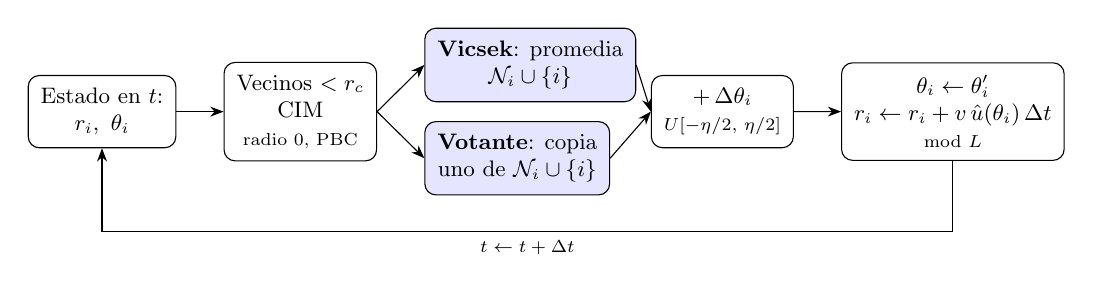
\begin{tikzpicture}[>=Stealth, font=\small, scale=0.9,
        every node/.append style={scale=0.9},
        caja/.style={draw, rounded corners, align=center, inner sep=5pt},
        regla/.style={caja, fill=blue!10}]
      \node[caja] (estado) {Estado en $t$:\\ $\vect{r}_i,\ \theta_i$};
      \node[caja, right=0.6cm of estado] (cim)
        {Vecinos $< r_c$\\ CIM\\ {\scriptsize radio $0$, PBC}};
      \node[regla, above right=0.12cm and 0.6cm of cim.east, anchor=south west] (vicsek)
        {\textbf{Vicsek}: promedia\\ $\mathcal{N}_i \cup \{i\}$};
      \node[regla, below right=0.12cm and 0.6cm of cim.east, anchor=north west] (voter)
        {\textbf{Votante}: copia\\ uno de $\mathcal{N}_i \cup \{i\}$};
      \node[caja] (ruido) at ($(vicsek.east)!0.5!(voter.east) + (1.4,0)$)
        {$+\,\Delta\theta_i$\\ {\scriptsize $U[-\eta/2,\,\eta/2]$}};
      \node[caja, right=0.6cm of ruido] (mover)
        {$\theta_i \leftarrow \theta_i'$\\
         $\vect{r}_i \leftarrow \vect{r}_i + v\,\hat{\vect{u}}(\theta_i)\,\Delta t$\\
         {\scriptsize mod $L$}};
      \draw[->] (estado) -- (cim);
      \draw[->] (cim.east) -- (vicsek.west);
      \draw[->] (cim.east) -- (voter.west);
      \draw[->] (vicsek.east) -- (ruido.west);
      \draw[->] (voter.east) -- (ruido.west);
      \draw[->] (ruido) -- (mover);
      \draw[->] (mover.south) -- ++(0,-1.0) -| (estado.south)
        node[pos=0.25, below, font=\scriptsize] {$t \leftarrow t + \Delta t$};
    \end{tikzpicture}
    \caption{Paso temporal del motor. $\hat{\vect{u}}(\theta)=(\cos\theta,\sin\theta)$
    y $\theta_i'$ es la dirección nueva antes de reemplazar la anterior.}
    \label{fig:motor}
\end{figure}

El cálculo simultáneo usa dos arreglos de ángulos. De esta forma, ninguna
partícula utiliza una dirección ya actualizada dentro del mismo paso. La grilla
del CIM tiene $M=10$ celdas por lado; como las partículas son puntuales,
$L/M=r_c=1$ permite revisar la celda propia y las ocho adyacentes. Para obtener
las componentes conexas se aplica una estructura union-find a los pares de
vecinos entregados por el CIM. En cada paso el motor guarda en archivos de
texto el estado, la polarización, la fracción del cluster más grande y el
tiempo de la llamada al CIM.

\section{Simulaciones}

\subsection{Sistema estudiado}

La densidad del sistema particular se definió como
\begin{equation}
    \rho = \frac{N}{L^2},
    \label{eq:density}
\end{equation}
donde $N$ es la cantidad de partículas y $L$ el lado de la caja. La
Fig.~\ref{fig:sistema} esquematiza el sistema y la
Tabla~\ref{tab:parametros} resume la configuración común a ambos modelos. Se
usaron 15 amplitudes de ruido entre $0$ y $6{,}28$ rad. Para cada punto se
ejecutaron 50 realizaciones con semillas distintas.

\begin{figure}[H]
    \centering
    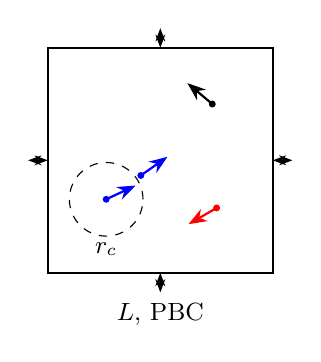
\begin{tikzpicture}[scale=0.55, >=Stealth]
      \draw[thick] (0,0) rectangle (5.2,5.2);
      \draw[<->, dashed] (-0.45,2.6) -- (0,2.6);
      \draw[<->, dashed] (5.2,2.6) -- (5.65,2.6);
      \draw[<->, dashed] (2.6,-0.45) -- (2.6,0);
      \draw[<->, dashed] (2.6,5.2) -- (2.6,5.65);
      \draw[dashed] (1.35,1.7) circle (0.85);
      \fill[blue] (1.35,1.7) circle (0.08);
      \draw[->, thick, blue] (1.35,1.7) -- ++(25:0.75);
      \fill[blue] (2.15,2.25) circle (0.08);
      \draw[->, thick, blue] (2.15,2.25) -- ++(35:0.75);
      \fill[red] (3.9,1.5) circle (0.08);
      \draw[->, thick, red] (3.9,1.5) -- ++(210:0.75);
      \fill[black] (3.8,3.9) circle (0.08);
      \draw[->, thick, black] (3.8,3.9) -- ++(140:0.75);
      \node[font=\small] at (1.35,0.55) {$r_c$};
      \node[font=\small] at (2.6,-0.95) {$L$, PBC};
    \end{tikzpicture}
    \caption{Sistema simulado: caja cuadrada de lado $L$ con condiciones
    periódicas de contorno (PBC). Cada flecha es la velocidad de una partícula
    puntual; el círculo de radio $r_c$ delimita la vecindad de la partícula
    azul, que en este ejemplo tiene un vecino.}
    \label{fig:sistema}
\end{figure}

\begin{table}[!htb]
    \centering
    \begin{tabular}{ll}
        \toprule
        Parámetro & Valor \\
        \midrule
        Lado de la caja, $L$ & $10$ m \\
        Radio de interacción, $r_c$ & $1$ m \\
        Rapidez, $v$ & $0{,}03$ m/s \\
        Paso temporal, $\Delta t$ & $1$ s \\
        Densidades principales, $\rho$ & $2$; $4$; $8$ \\
        Densidades complementarias, $\rho$ & $1/(3\pi)$; $1/(2\pi)$; $1/\pi$ \\
        Ruido, $\eta$ (rad) & $0$; $0{,}25$; $0{,}5$; $0{,}75$; $1$; $1{,}5$; \\
        & $2$; $2{,}5$; $3$; $3{,}5$; $4$; $4{,}5$; $5$; $5{,}5$; $6{,}28$ \\
        Realizaciones por punto & $50$ \\
        Duración, $T$ & $2000$ s \\
        \bottomrule
    \end{tabular}
    \caption{Parámetros de las simulaciones, comunes a ambos modelos.}
    \label{tab:parametros}
\end{table}

Los valores de la Tabla~\ref{tab:parametros} rigen para todas las corridas y
todas las figuras de este informe; solo se indicará cuando un parámetro varíe
respecto de ella. Las densidades complementarias se agregaron para estudiar
el sistema por debajo de $\rho=2$.

\subsection{Observables y protocolo de medición}

La polarización es el módulo de la velocidad media normalizado por la rapidez
individual:
\begin{equation}
    \va(t) = \frac{\left|\sum_{i=1}^{N}\vect{v}_i(t)\right|}{N v}.
    \label{eq:polarization}
\end{equation}
Aquí $\vect{v}_i(t)$ es la velocidad de la partícula $i$ en el instante $t$ y
$v=|\vect{v}_i(t)|$, común a todas las partículas. Por lo tanto, la
Ec.~\eqref{eq:polarization} da $\va\simeq1$ cuando el sistema está polarizado,
es decir, cuando todas las partículas se mueven en direcciones similares, y
$\va\simeq0$ cuando no lo está: las direcciones se reparten en todo el
círculo y la suma de velocidades se cancela.

Se definió un cluster como una componente conexa del grafo cuyos nodos son las
partículas y cuyas aristas unen vecinos. Si $N_{\max}(t)$ es la cantidad de
partículas en la componente más grande en el instante $t$, su fracción es
\begin{equation}
    S(t) = \frac{N_{\max}(t)}{N}.
    \label{eq:giant-cluster}
\end{equation}
En la Ec.~\eqref{eq:giant-cluster}, el valor $S=1$ corresponde a una única
componente conectada.

El valor escalar de cada realización es el promedio temporal del observable
sobre la segunda mitad de la corrida. Las evoluciones temporales de la
Sección~\ref{sec:resultados} verifican que el estado estacionario empieza
antes de ese corte en todos los casos mostrados:
\begin{equation}
    \overline{A} = \frac{1}{n}\sum_{t\,\geq\,T/2} A(t),
    \qquad A\in\{\va,S\},
    \label{eq:stationary-average}
\end{equation}
donde $T$ es la duración de la corrida y $n$ la cantidad de instantes con
$t\geq T/2$. Cada punto de las curvas de la Sección~\ref{sec:resultados} es
el promedio de $\overline{A}$ sobre las 50 realizaciones y su barra de error,
el desvío estándar entre realizaciones.

\section{Resultados}
\label{sec:resultados}

Los resultados se presentan en el mismo orden que el estudio: primero se
caracteriza el modelo de Vicsek y luego se repite el análisis para el modelo de
votante. En ambos casos se muestra la dinámica, se valida el promedio temporal
y se estudian \va\ y $S$ en función del ruido.

\subsection{Modelo de Vicsek}

\subsubsection{Dinámica característica}

La Fig.~\ref{fig:anim-vicsek} compara dos instantes de las animaciones de
Vicsek para $\rho=2$, la menor de las densidades principales y por lo tanto la
que permite distinguir los vectores individuales. Los vectores se colorean
según su dirección. Con $\eta=0{,}5$ rad casi todas las partículas comparten
el mismo color y la polarización instantánea es $0{,}984$. Con $\eta=4$ rad
conviven direcciones de todo el círculo y la polarización de ese instante cae
a $0{,}043$. El cluster más grande abarca todo el sistema en el primer caso
y $S=0{,}995$ en el segundo.

\begin{figure}[H]
    \centering
    \begin{minipage}{\figwpair}
        \centering
        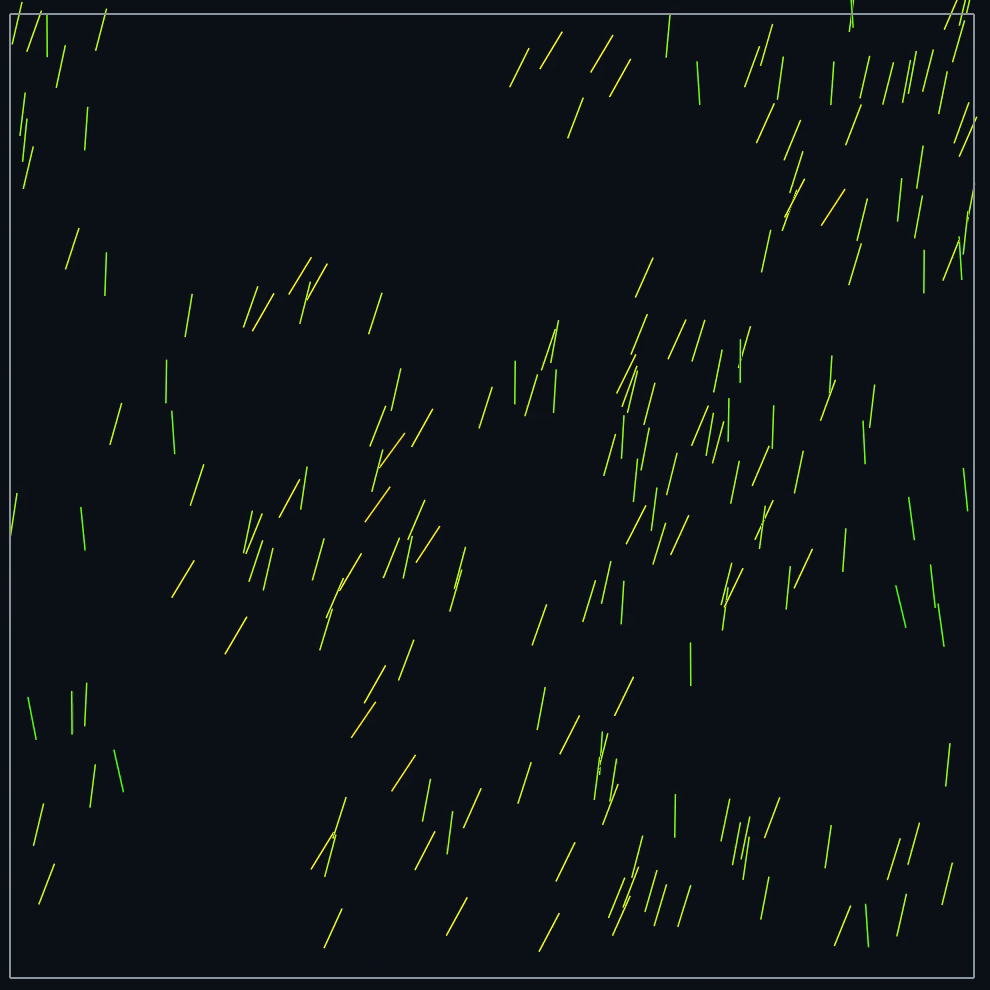
\includegraphics[width=\linewidth]{anim_vicsek_rho2_eta05.png}\\
        (a) $\eta=0{,}5$ rad. \yt{P-lkSdXIhaI}
    \end{minipage}\hfill
    \begin{minipage}{\figwpair}
        \centering
        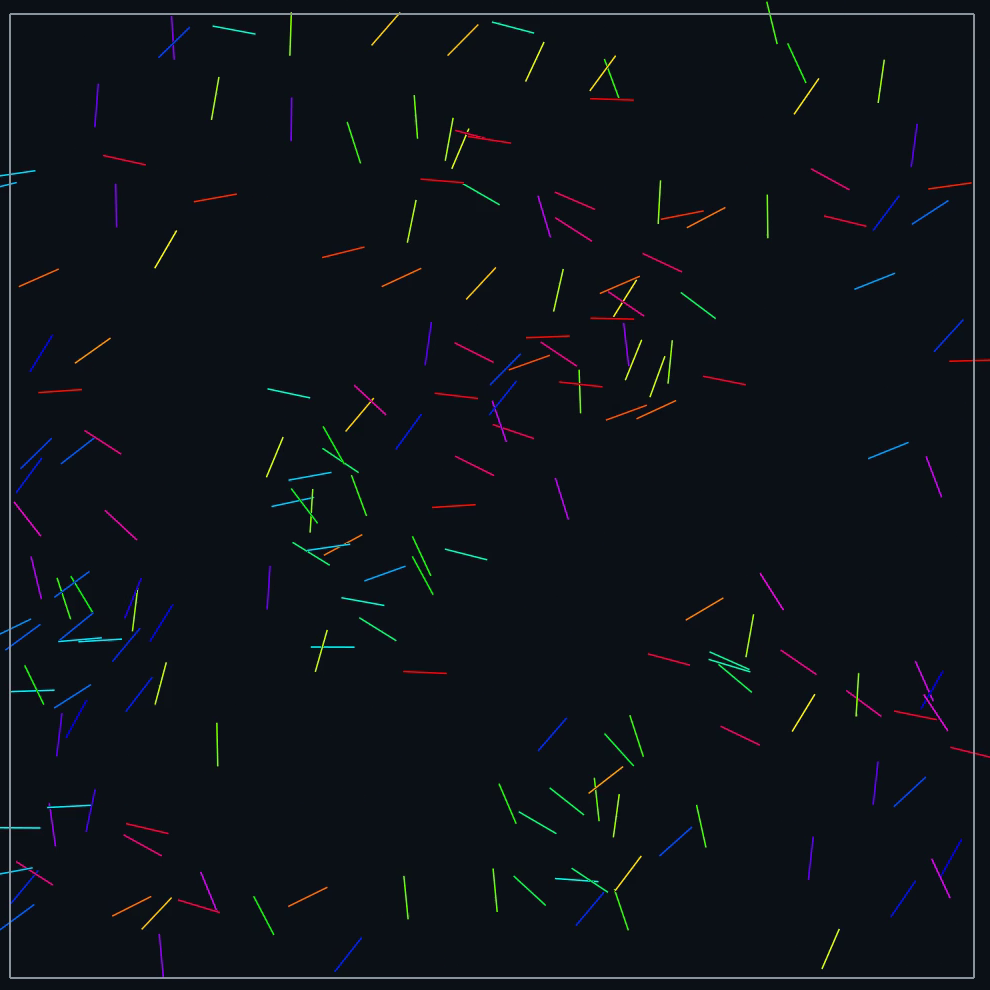
\includegraphics[width=\linewidth]{anim_vicsek_rho2_eta4.png}\\
        (b) $\eta=4$ rad. \yt{ez4dm6Y6-3w}
    \end{minipage}
    \caption{Fotogramas en $t=1500$ s de una realización del modelo de Vicsek
    para $\rho=2$.
    Cada segmento representa la velocidad de una partícula y su color, el
    ángulo de movimiento. Debajo de cada panel, el enlace a la animación
    completa.}
    \label{fig:anim-vicsek}
\end{figure}


\subsubsection{Polarización}

La evolución de la Fig.~\ref{fig:evol-va-vicsek} muestra que el transitorio de
Vicsek termina antes de $t=150$ s para los tres ruidos (líneas verticales de
trazos, una por curva), muy antes del corte en $T/2=1000$ s de la
Ec.~\eqref{eq:stationary-average}. Sin ruido, la polarización llega a uno; para
$\eta=0{,}5$ rad se estabiliza cerca del mismo valor y para $\eta=2$ rad
alcanza un nivel menor. Los promedios estacionarios de esas tres curvas,
calculados con la Ec.~\eqref{eq:stationary-average} y promediados sobre las
50 realizaciones, son $\langle\overline{\va}\rangle=1{,}000$;
$0{,}9862\pm0{,}0007$ y $0{,}783\pm0{,}007$. Promediar el último $10\%$ de
cada corrida en lugar de la segunda mitad cambia los 180 puntos del barrido en
$0{,}14$ desvíos en mediana y a lo sumo $0{,}7$: el resultado no depende de
dónde se corte.

\begin{figure}[H]
    \centering
    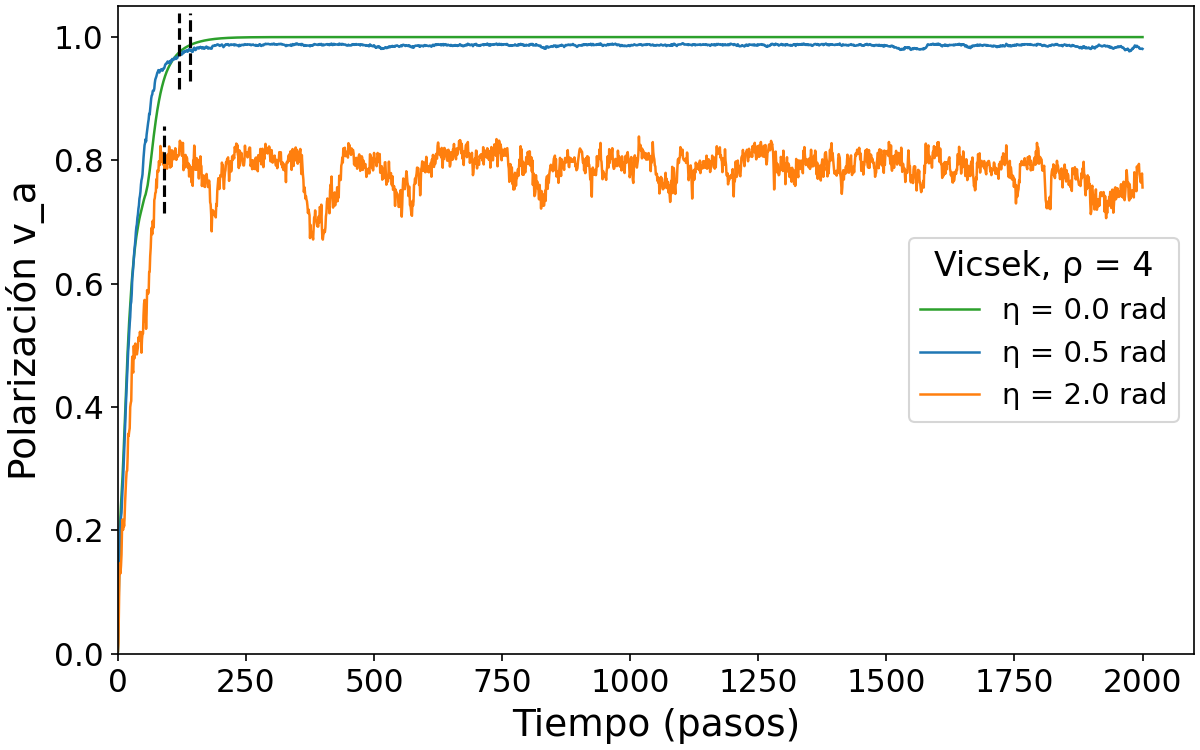
\includegraphics[width=\figw]{evolucion_va_vicsek_rho4.png}
    \caption{Evolución de la polarización en el modelo de Vicsek para
    $\rho=4$ y una realización. Cada línea vertical de trazos marca el
    comienzo del régimen estacionario de la curva de su color.}
    \label{fig:evol-va-vicsek}
\end{figure}

La Fig.~\ref{fig:va-eta-vicsek} extiende la comparación a todo el barrido. En
las densidades principales, aumentar $\rho$ desplaza la pérdida de orden hacia
ruidos mayores. Para $\rho=4$, por ejemplo, se obtuvo
$\langle\overline{\va}\rangle=1{,}000$ en $\eta=0$,
$0{,}783\pm0{,}007$ en $\eta=2$ rad y $0{,}0443\pm0{,}0008$ en
$\eta=6{,}28$ rad. Las densidades complementarias pierden orden con ruidos
menores y, con el ruido máximo, su polarización queda tanto más alta cuanto
menor es la densidad.

\begin{figure}[H]
    \centering
    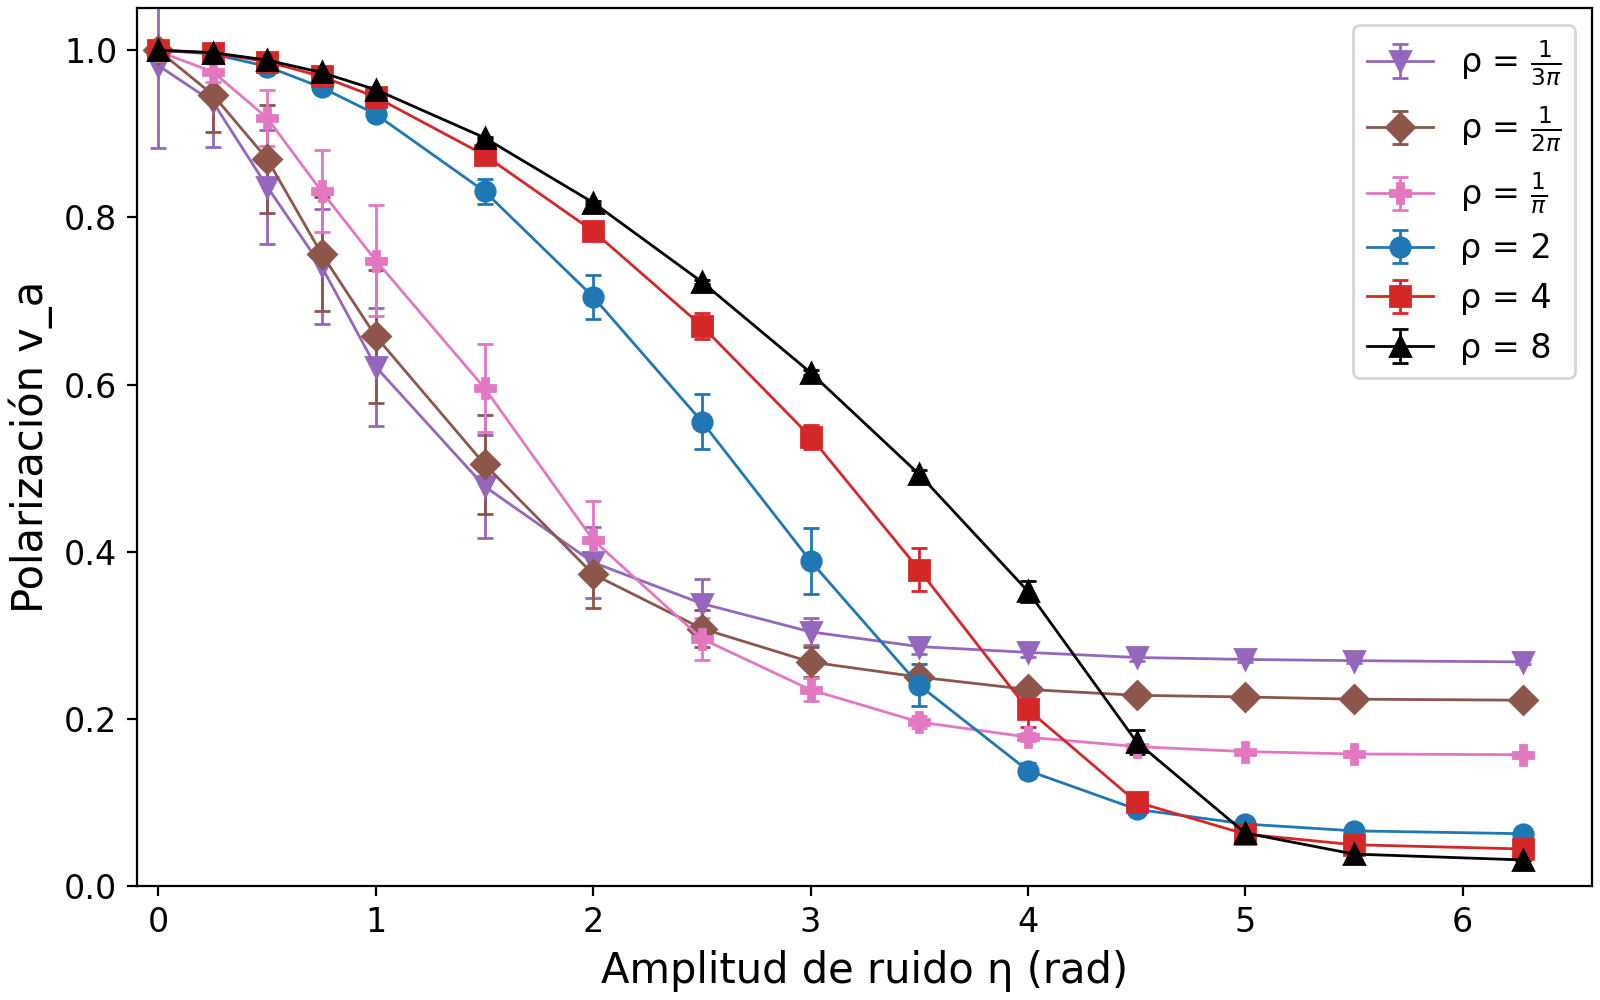
\includegraphics[width=\figw]{vicsek_va_vs_eta.png}
    \caption{Polarización estacionaria en función del ruido para el modelo de
    Vicsek. Además de las densidades principales se muestran las tres
    densidades complementarias.}
    \label{fig:va-eta-vicsek}
\end{figure}


\subsubsection{Conectividad}

La Fig.~\ref{fig:evol-s-vicsek} muestra la evolución de $S$ para $\rho=2$,
la densidad principal donde más varía, y para $\rho=1/\pi$, una de las
complementarias. En $\rho=2$ las tres curvas son estacionarias desde el
inicio: aparecen fragmentaciones breves, pero el cluster más grande sigue
conteniendo a la mayor parte del sistema; para $\rho=4$ y $8$ se mantiene en
uno durante toda la corrida. En $\rho=1/\pi$ el transitorio es más largo: sin
ruido el sistema se reúne en un único cluster en $t\simeq400$ s, con
$\eta=0{,}5$ rad $S$ es estacionario desde $t\simeq140$ s y oscila entre
$0{,}5$ y $1$, y con $\eta=2$ rad lo es desde $t\simeq130$ s y oscila
alrededor de $0{,}4$. Todos esos inicios quedan antes del corte de la
Ec.~\eqref{eq:stationary-average}, que es $1000$ s para $\rho=2$ y $2500$ s
para $\rho=1/\pi$. Los promedios estacionarios sobre las 50 realizaciones son
$\langle\overline{S}\rangle=0{,}9999\pm0{,}0007$; $0{,}994\pm0{,}006$ y
$0{,}98\pm0{,}01$ para $\rho=2$, y $0{,}98\pm0{,}08$; $0{,}81\pm0{,}09$ y
$0{,}48\pm0{,}07$ para $\rho=1/\pi$.

\begin{figure}[H]
    \centering
    \begin{minipage}{\figwpair}
        \centering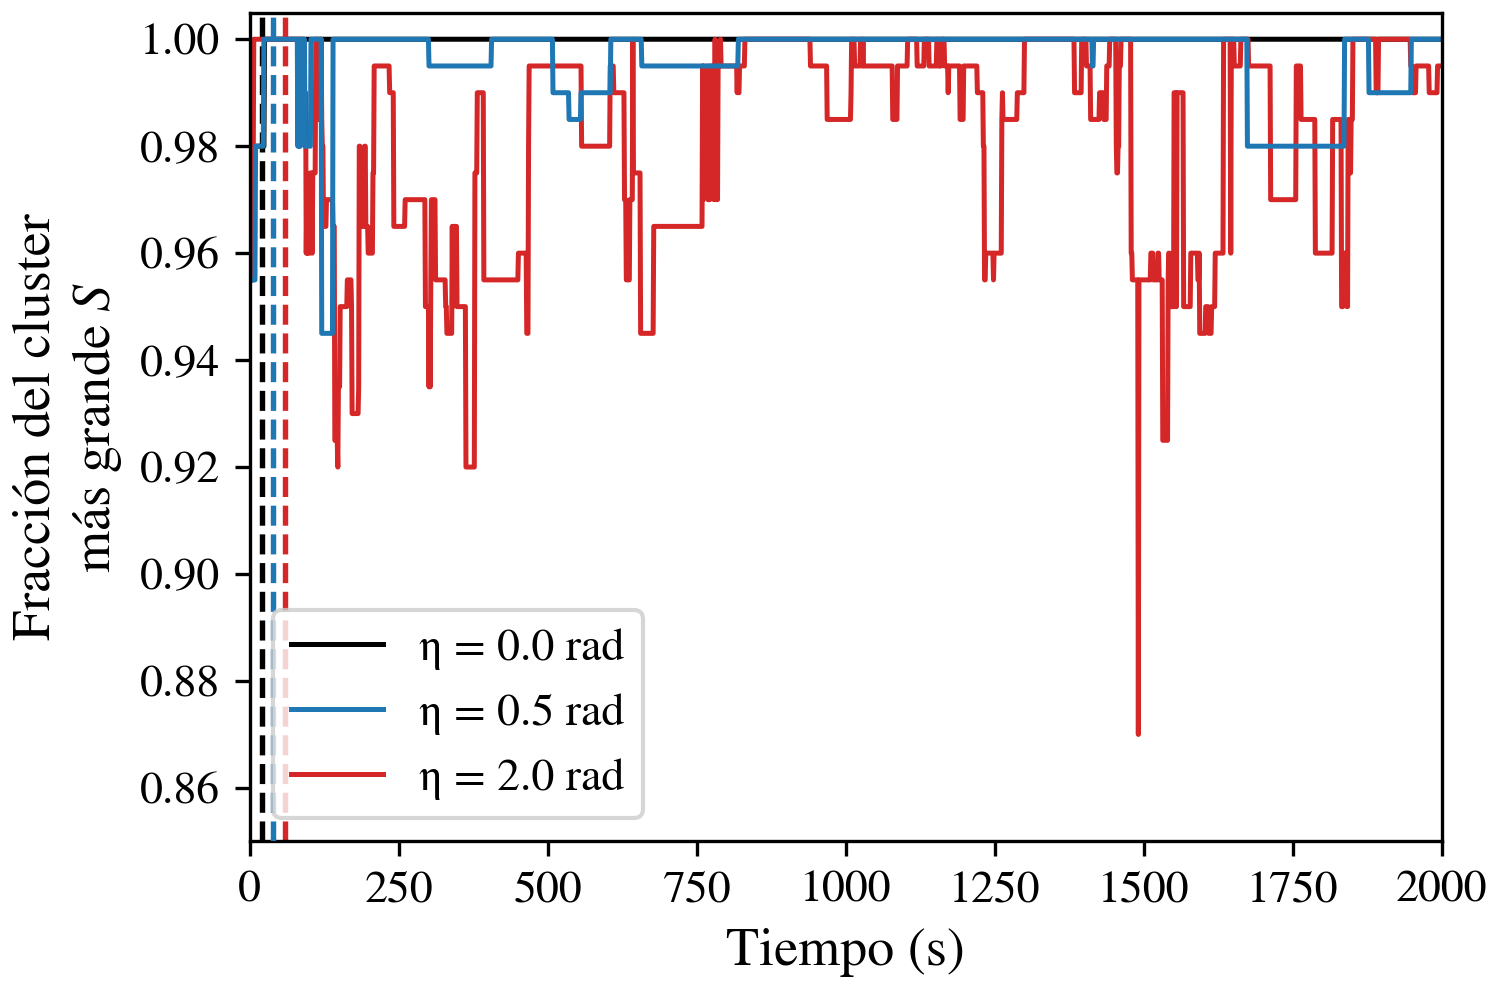
\includegraphics[width=\linewidth]{evolucion_s_vicsek_rho2.png}\\
        (a) $\rho=2$, $T=2000$ s.
    \end{minipage}\hfill
    \begin{minipage}{\figwpair}
        \centering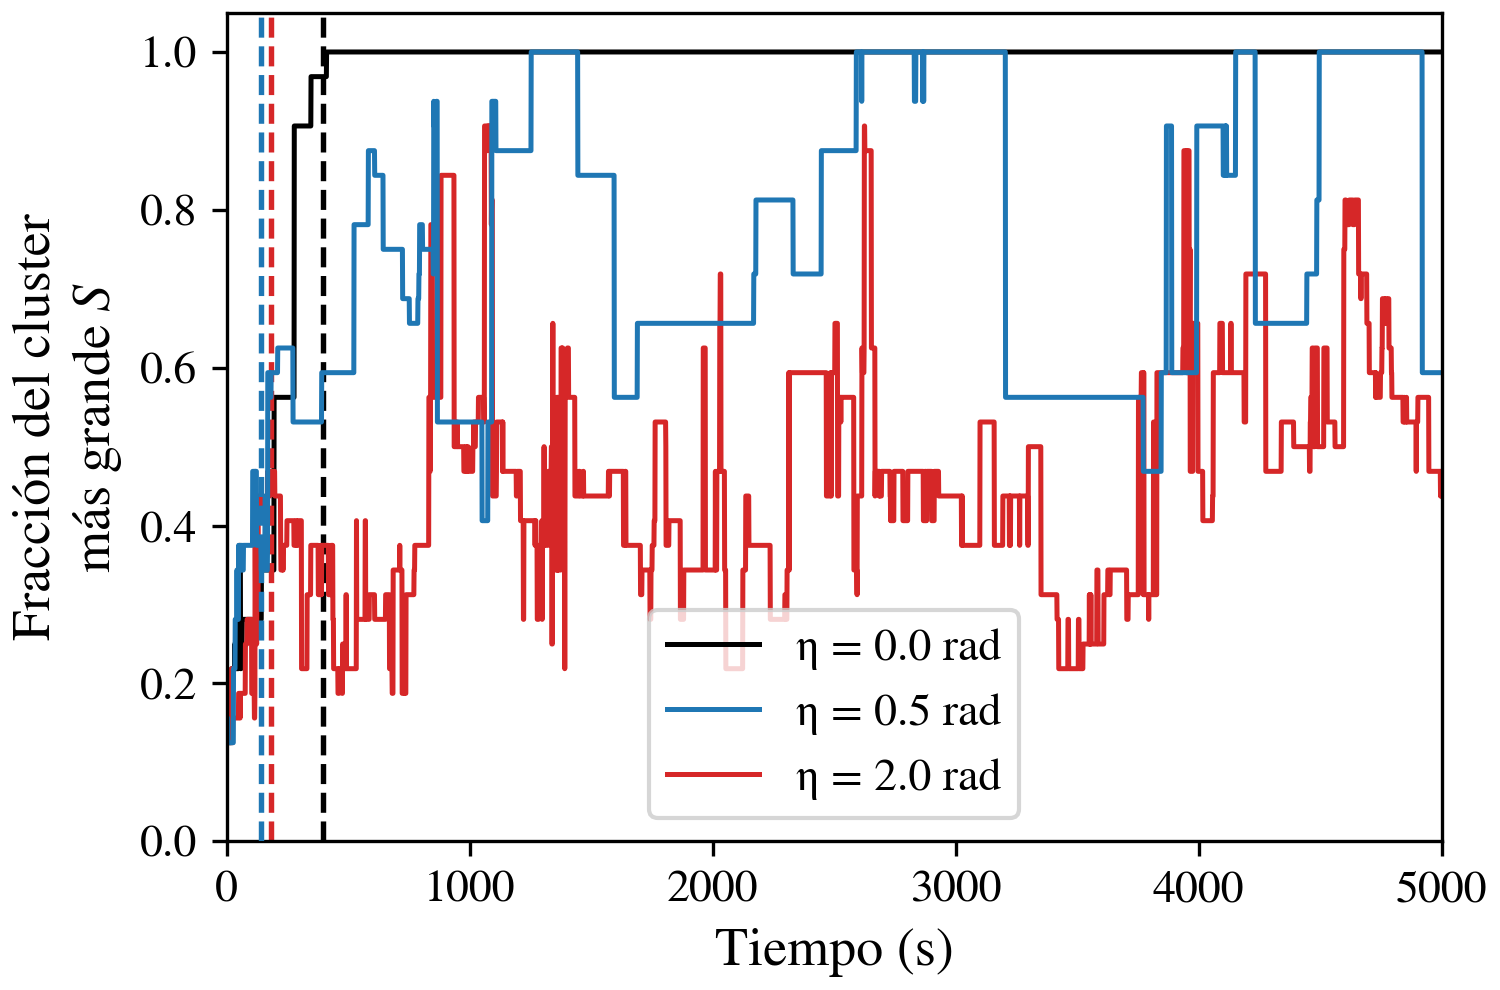
\includegraphics[width=\linewidth]{evolucion_s_vicsek_rho0.3183.png}\\
        (b) $\rho=1/\pi$, $T=5000$ s.
    \end{minipage}
    \caption{Evolución de la fracción del cluster más grande para Vicsek. Cada
    panel corresponde a una realización y compara $\eta=0$, $0{,}5$ y $2$
    rad. Cada línea vertical de trazos marca el comienzo del régimen
    estacionario de la curva de su color; en (a) las tres empiezan en $t=0$
    y se dibujan levemente corridas para que se distingan. En (a) el eje
    vertical se acotó al intervalo donde varían los datos.}
    \label{fig:evol-s-vicsek}
\end{figure}

El barrido de la Fig.~\ref{fig:s-eta-vicsek} confirma que, para $\rho\geq2$,
$S$ se mantiene cerca de uno tanto cuando el sistema está polarizado como
cuando no lo está. El
mínimo medio fue $0{,}96\pm0{,}01$ para $\rho=2$, en $\eta=3$ a $3{,}5$ rad,
donde \va\ cae por debajo de $0{,}4$; a ambos lados $S$ vuelve a $0{,}99$.
Para $\rho=4$ y $8$ el mínimo superó $0{,}998$. En cambio, para
$\rho\leq1/\pi$ la fracción del cluster más grande disminuye con el ruido y
se aproxima a un nivel bajo a partir de $\eta\simeq4$ rad. En $\rho=1/\pi$,
$S$ pasó de $0{,}98\pm0{,}08$ en $\eta=0$ a $0{,}16\pm0{,}04$ en
$\eta=6{,}28$ rad.

\begin{figure}[H]
    \centering
    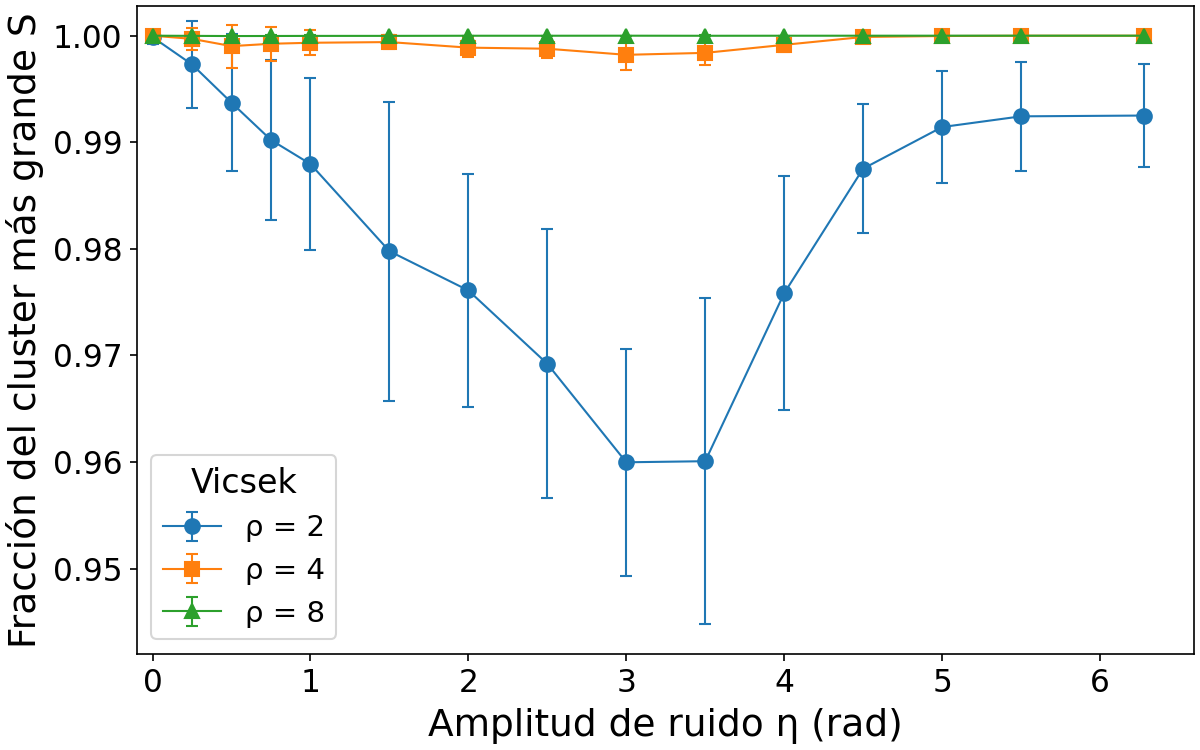
\includegraphics[width=\figw]{vicsek_s_vs_eta.png}
    \caption{Fracción estacionaria del cluster más grande en función del ruido
    para el modelo de Vicsek.}
    \label{fig:s-eta-vicsek}
\end{figure}

La relación entre ambos observables se muestra en la
Fig.~\ref{fig:va-s-vicsek}. En el panel derecho, con $\rho=2$, $4$ y
$8$, los puntos forman una columna en $S\simeq1$ mientras \va\ recorre casi
todo su intervalo: para estas densidades el cluster más grande abarca casi todo
el sistema con cualquier ruido, mientras que la polarización sí depende del
ruido. En el panel izquierdo, con las densidades complementarias, ambos
observables aumentan juntos: la amplitud del ruido modifica simultáneamente
la orientación y la estructura espacial.

\begin{figure}[H]
    \centering
    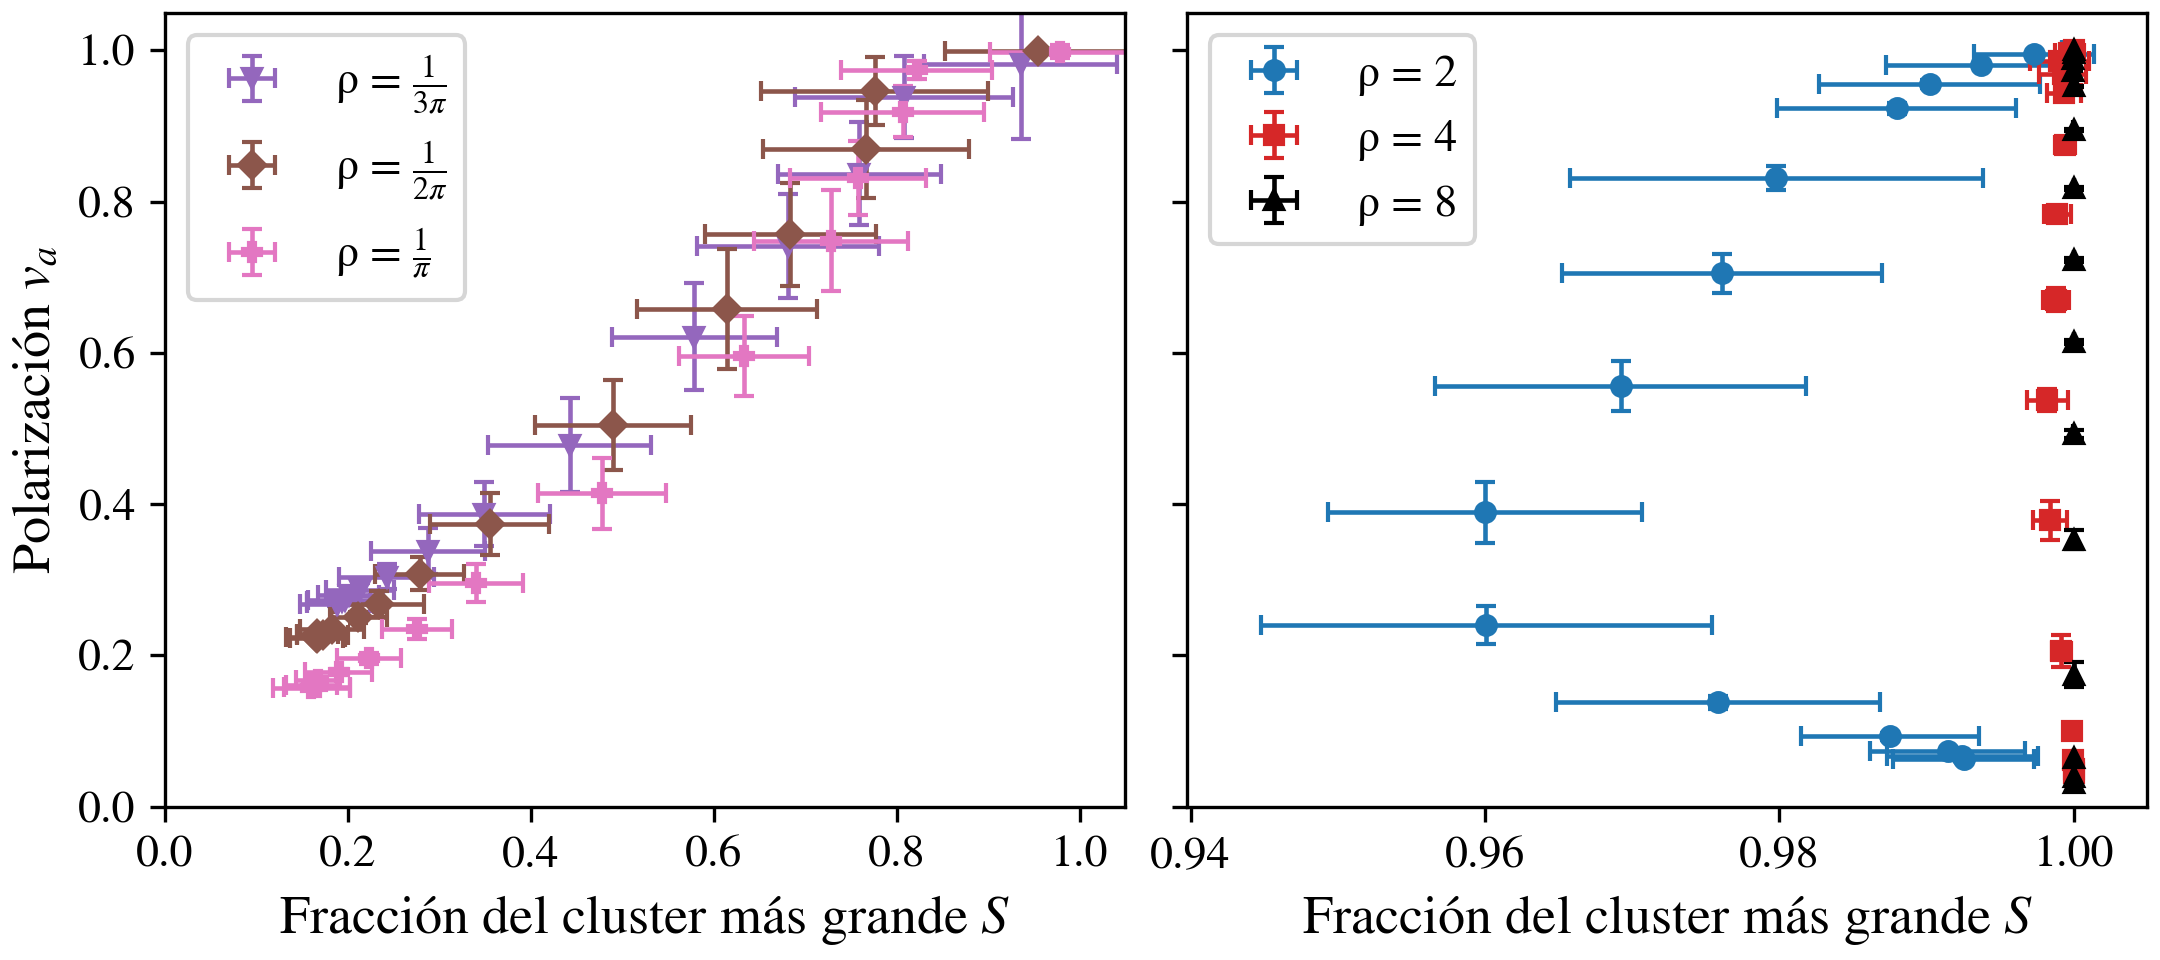
\includegraphics[width=0.88\textwidth]{va_vs_s_vicsek.png}
    \caption{Polarización en función de la fracción del cluster más grande para
    Vicsek. Cada punto corresponde a un valor de ruido y las barras son los
    desvíos estándar de $S$ (horizontales) y \va\ (verticales). En el panel
    derecho el eje horizontal está acotado a los datos.}
    \label{fig:va-s-vicsek}
\end{figure}


\subsection{Modelo de votante}

\subsubsection{Dinámica característica}

La Fig.~\ref{fig:anim-voter} repite la misma densidad y los mismos dos ruidos
para el votante, de modo que cada panel se compara con el de Vicsek. Con
$\eta=0{,}5$ rad, donde Vicsek alcanza $0{,}984$, el votante ya muestra
direcciones de todo el círculo y su polarización en ese instante es
$0{,}553$. Con $\eta=4$ rad baja a $0{,}101$. En ambos casos $S=1{,}000$.

\begin{figure}[H]
    \centering
    \begin{minipage}{\figwpair}
        \centering
        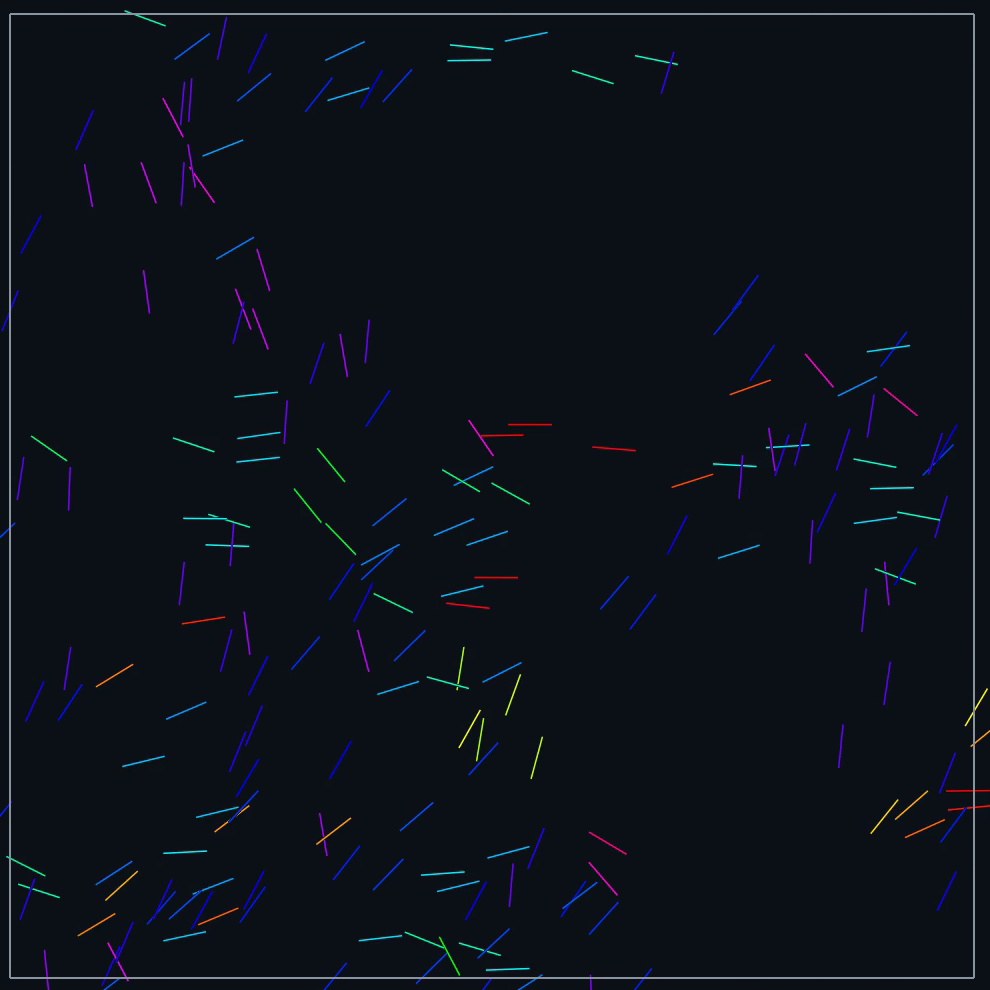
\includegraphics[width=\linewidth]{anim_voter_rho2_eta05.png}\\
        (a) $\eta=0{,}5$ rad. \yt{tHQbmPHvScs}
    \end{minipage}\hfill
    \begin{minipage}{\figwpair}
        \centering
        
\includegraphics[width=\linewidth]{anim_voter_rho2_eta4.png}\\
        (b) $\eta=4$ rad. \yt{UtGcnTB9IRE}
    \end{minipage}
    \caption{Fotogramas en $t=1500$ s de una realización del modelo de votante
    para $\rho=2$. La densidad, los ruidos y la representación son los mismos
    que en la Fig.~\ref{fig:anim-vicsek}. Debajo de cada panel, el enlace a la
    animación completa.}
    \label{fig:anim-voter}
\end{figure}


\subsubsection{Polarización}

La evolución temporal de la Fig.~\ref{fig:evol-va-voter} difiere de Vicsek. La
corrida sin ruido alcanza $\va=1$ en $t\simeq320$ s y no vuelve a cambiar;
esas corridas se extendieron a $10000$ s porque el consenso tarda más
cuanto mayor es $N$, y la figura muestra sus primeros $2000$ s. Para
$\eta=0{,}5$ rad y $\eta=2$ rad el régimen estacionario comienza desde el
inicio: el sistema parte desordenado y se mantiene así. La realización con
$\eta=0{,}5$ rad oscila entre $0{,}1$ y $0{,}6$, pero alrededor de un valor
fijo: la media entre las 50 realizaciones fue $0{,}282$ en el tercer cuarto
de la corrida y $0{,}288$ en el último, y el desvío entre realizaciones
conserva esa dispersión. El corte en $T/2$ ($5000$ s sin ruido, $1000$ s en
los otros dos casos) cae dentro del estacionario de las tres curvas. Los
promedios estacionarios son $\langle\overline{\va}\rangle=1{,}000$;
$0{,}28\pm0{,}04$ y $0{,}079\pm0{,}003$.

\begin{figure}[H]
    \centering
    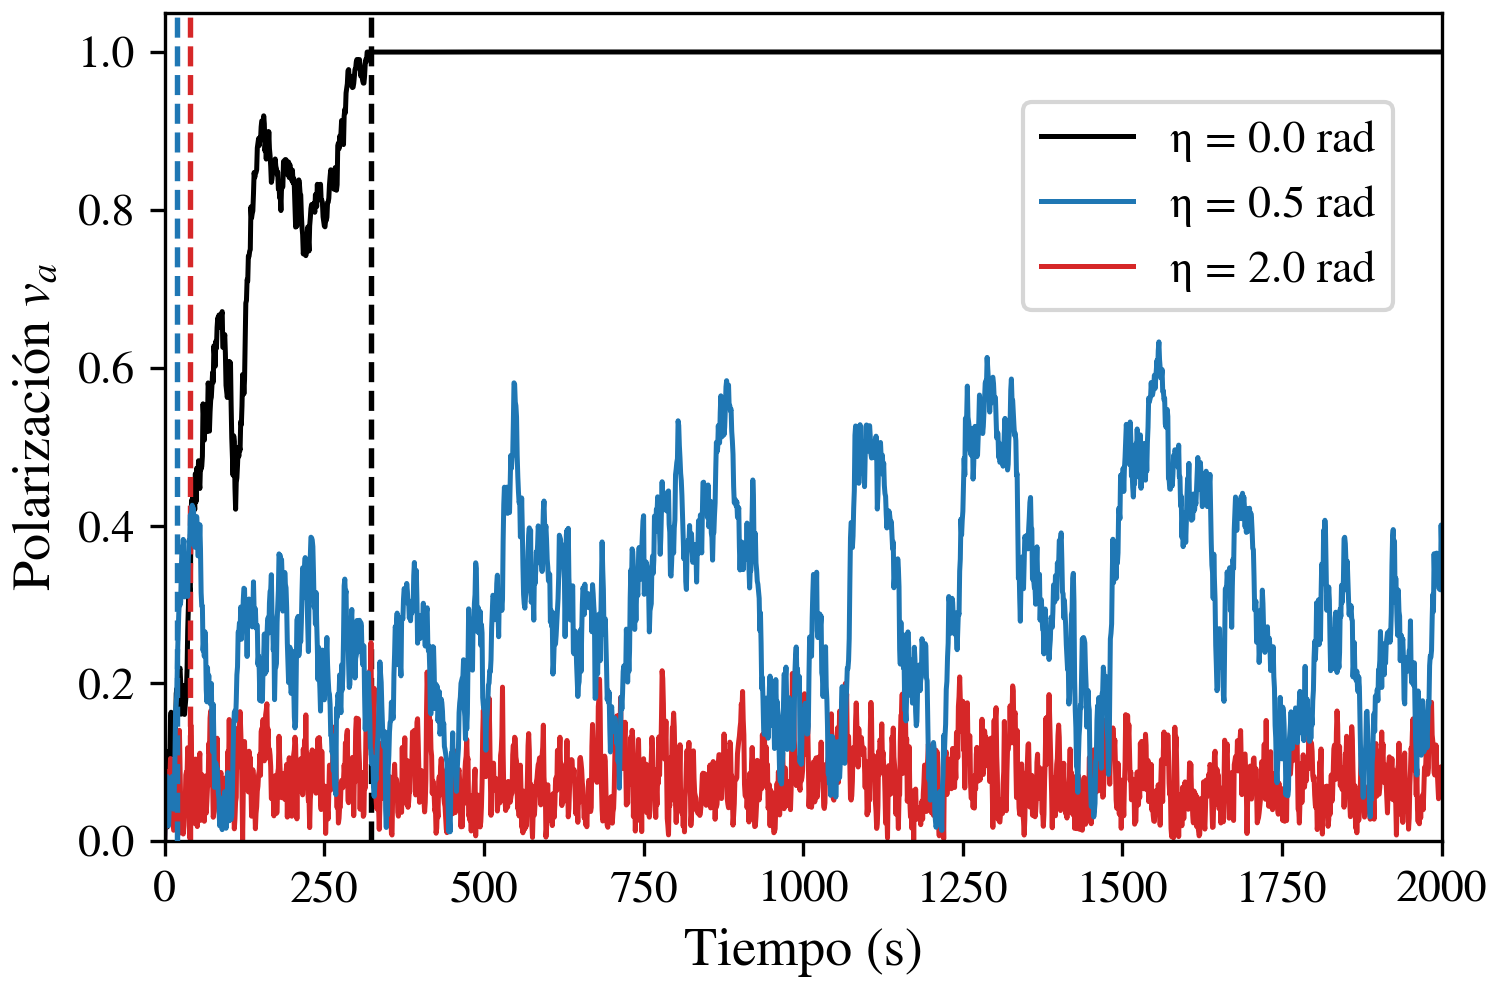
\includegraphics[width=\figw]{evolucion_va_voter_rho4.png}
    \caption{Evolución de la polarización en el modelo de votante para
    $\rho=4$ y una realización. Las líneas verticales de trazos marcan el
    comienzo del régimen estacionario de la curva de su color; las de
    $\eta=0{,}5$ y $2$ rad empiezan en $t=0$ y se dibujan levemente corridas
    para que se distingan.}
    \label{fig:evol-va-voter}
\end{figure}

El barrido completo se muestra en la Fig.~\ref{fig:va-eta-voter}. Todas las
densidades pierden el orden dentro del primer radián, mucho antes que en
Vicsek. La diferencia cualitativa con la Fig.~\ref{fig:va-eta-vicsek} es el
efecto de la densidad: en Vicsek aumentar $\rho$ desplaza la caída hacia ruidos
mayores, mientras que en el votante no la desplaza y, de hecho, la agudiza.
Para $\eta=0{,}25$ rad la polarización bajó de $0{,}6\pm0{,}1$ en $\rho=2$
a $0{,}53\pm0{,}08$ en $\rho=4$ y a $0{,}39\pm0{,}09$ en $\rho=8$,
mientras que en Vicsek, para el mismo ruido, subió de $0{,}9954\pm0{,}0009$
en $\rho=2$ a $0{,}99704\pm0{,}00008$ en $\rho=8$. El resultado es
consistente con la regla: promediar sobre los vecinos atenúa el ruido tanto
más cuanto más vecinos haya, pero copiar a uno solo no promedia nada, así que
agregar vecinos no aporta resistencia al ruido.

\begin{figure}[H]
    \centering
    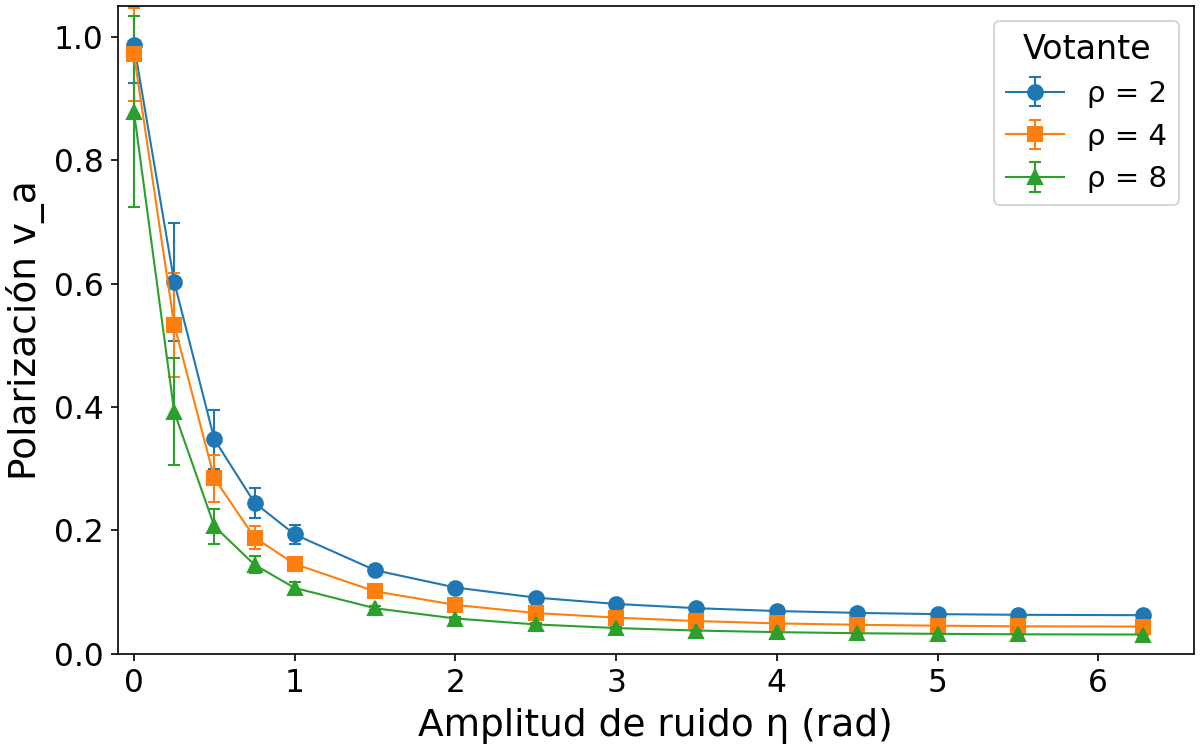
\includegraphics[width=\figw]{voter_va_vs_eta.png}
    \caption{Polarización estacionaria en función del ruido para el modelo de
    votante.}
    \label{fig:va-eta-voter}
\end{figure}

La comparación directa de la Fig.~\ref{fig:comparacion-va-voter} muestra que
copiar una sola dirección produce una pérdida de orden con ruidos mucho
menores que promediar todas las direcciones vecinas. Para $\rho=4$ y
$\eta=0{,}25$ rad, el votante alcanzó
$\langle\overline{\va}\rangle=0{,}53\pm0{,}08$, mientras que Vicsek
alcanzó $0{,}9966\pm0{,}0002$. En $\eta=6{,}28$ rad ambos modelos convergen
al mismo valor, $\va\simeq0{,}044$.

\begin{figure}[H]
    \centering
    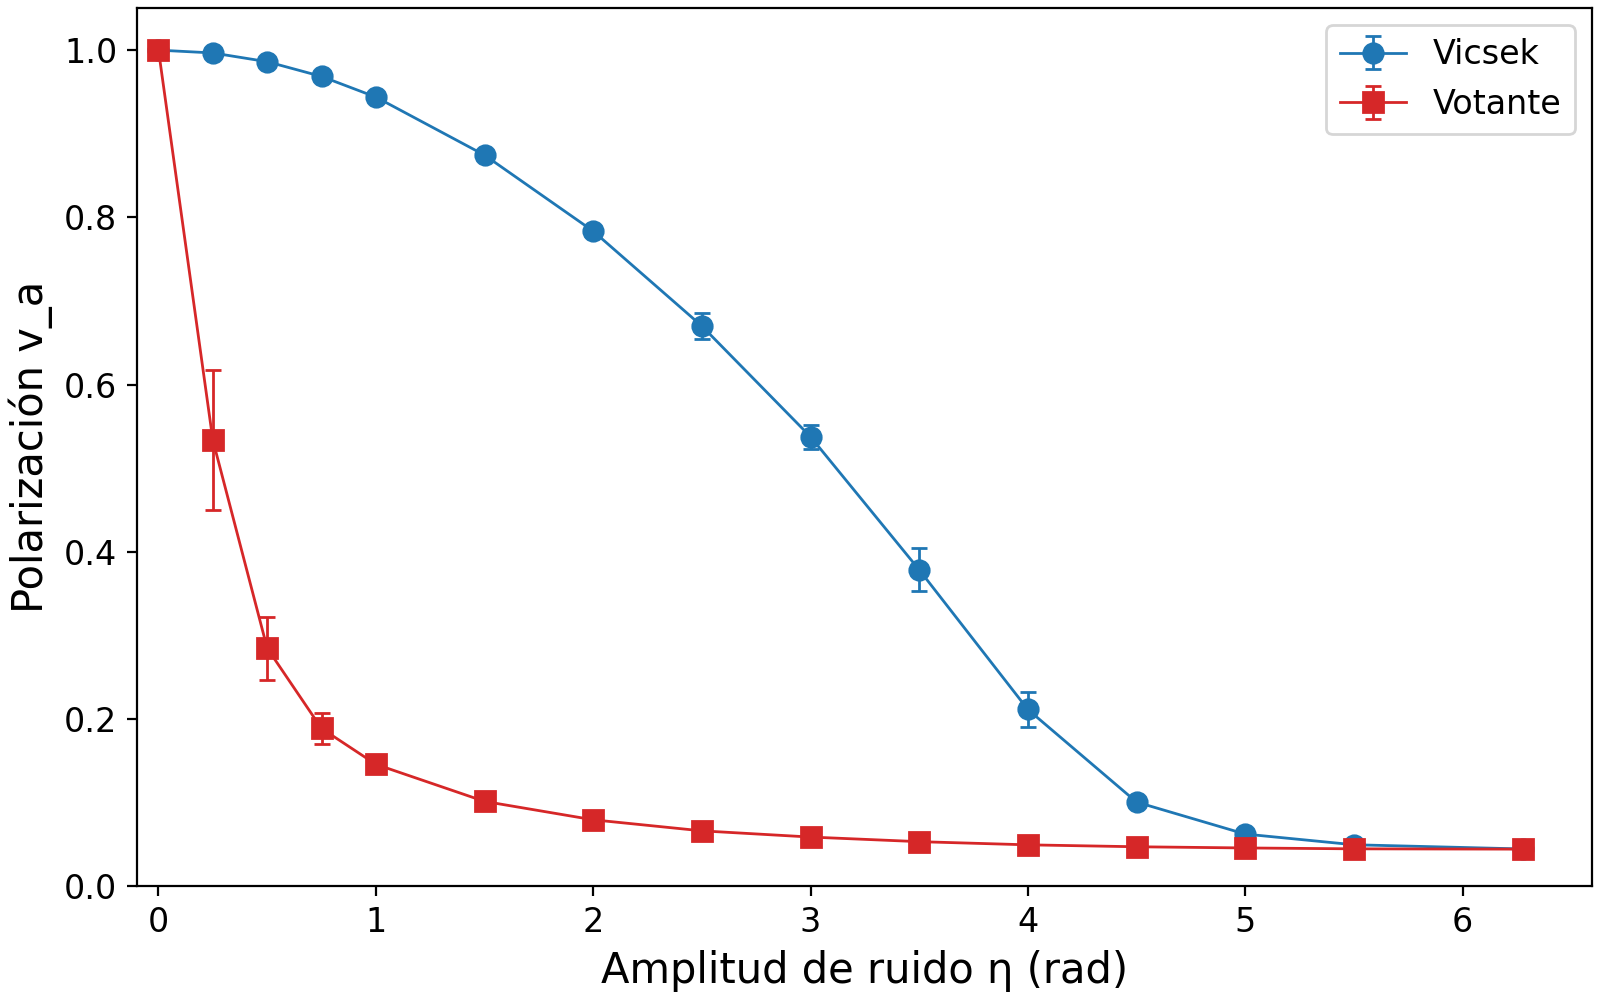
\includegraphics[width=\figw]{comparacion_va_vs_eta_rho4.png}
    \caption{Polarización estacionaria en función del ruido para Vicsek y
    votante con $\rho=4$.}
    \label{fig:comparacion-va-voter}
\end{figure}


\subsubsection{Conectividad}

La evolución de $S$ para el votante, presentada en la
Fig.~\ref{fig:evol-s-voter} para las mismas dos densidades que en Vicsek,
repite la estructura observada allí. En $\rho=2$ aparecen caídas breves y el
cluster más grande abarca prácticamente todo el sistema; las tres curvas son
estacionarias desde el inicio (la de $\eta=0$, desde $t\simeq50$ s). En
$\rho=1/\pi$, sin ruido el sistema queda en un único cluster en
$t\simeq900$ s; con $\eta=0{,}5$ rad $S$ es estacionario desde $t\simeq60$ s
y oscila entre $0{,}3$ y $0{,}9$, y con $\eta=2$ rad oscila alrededor de
$0{,}2$ desde el inicio, por debajo de Vicsek. El inicio más tardío,
$900$ s, sigue lejos del corte de $5000$ s de las corridas sin ruido; en las
demás el corte es $1000$ s ($\rho=2$) o $2500$ s ($\rho=1/\pi$). Los promedios
estacionarios son $\langle\overline{S}\rangle=0{,}99\pm0{,}04$;
$0{,}975\pm0{,}011$ y $0{,}987\pm0{,}006$ para $\rho=2$, y
$0{,}9\pm0{,}2$; $0{,}54\pm0{,}05$ y $0{,}22\pm0{,}03$ para $\rho=1/\pi$.

\begin{figure}[H]
    \centering
    \begin{minipage}{\figwpair}
        \centering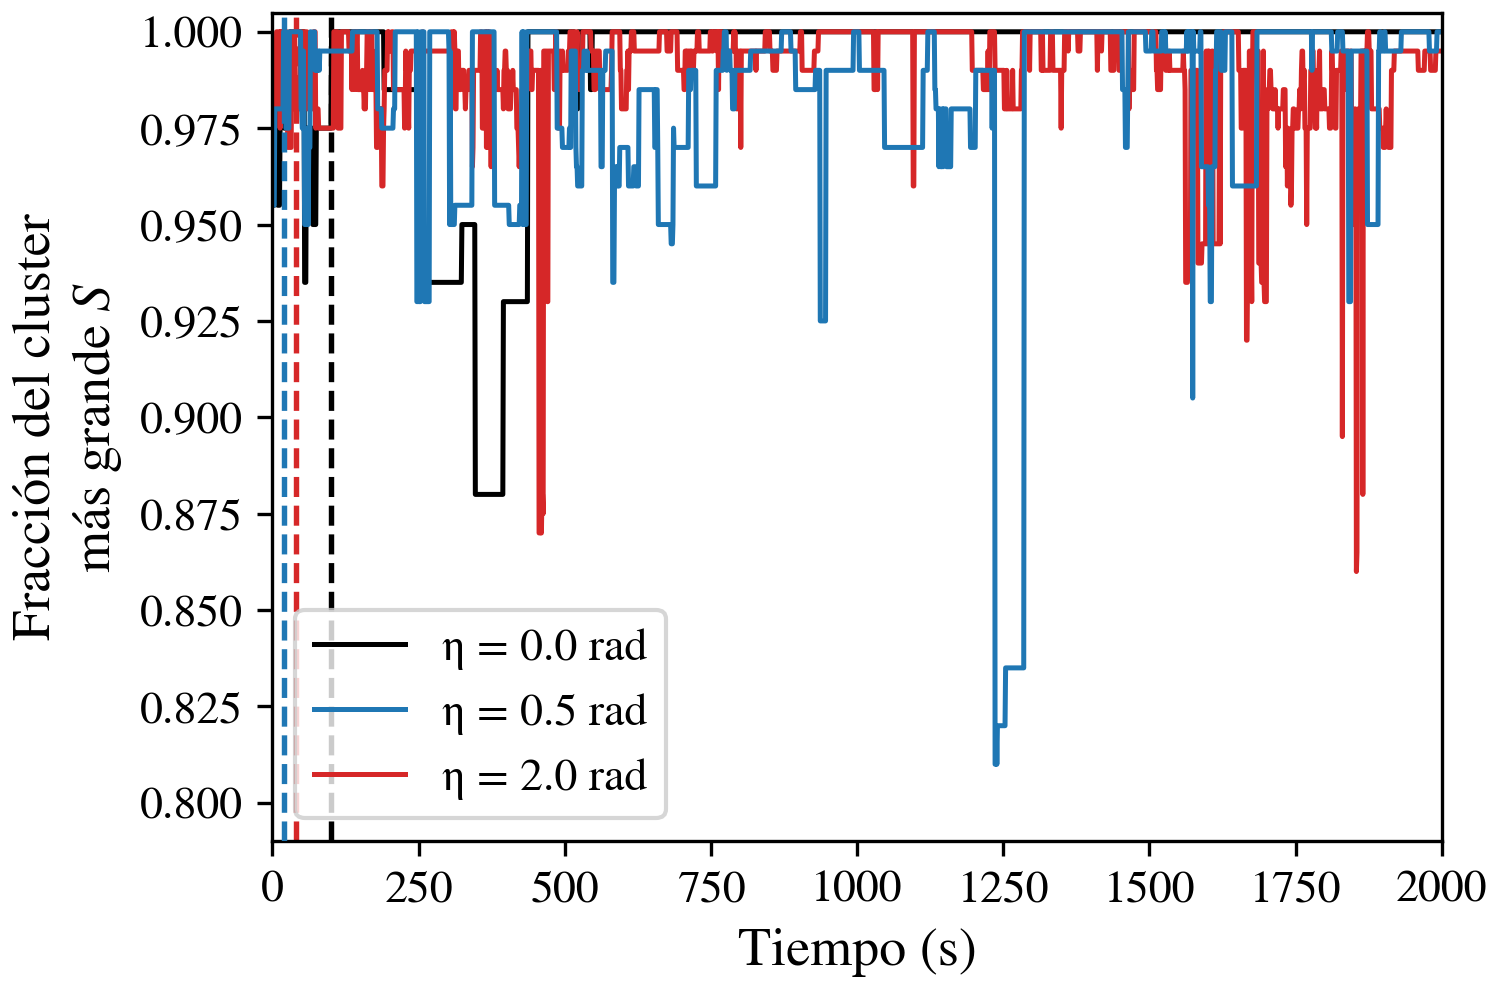
\includegraphics[width=\linewidth]{evolucion_s_voter_rho2.png}\\
        (a) $\rho=2$.
    \end{minipage}\hfill
    \begin{minipage}{\figwpair}
        \centering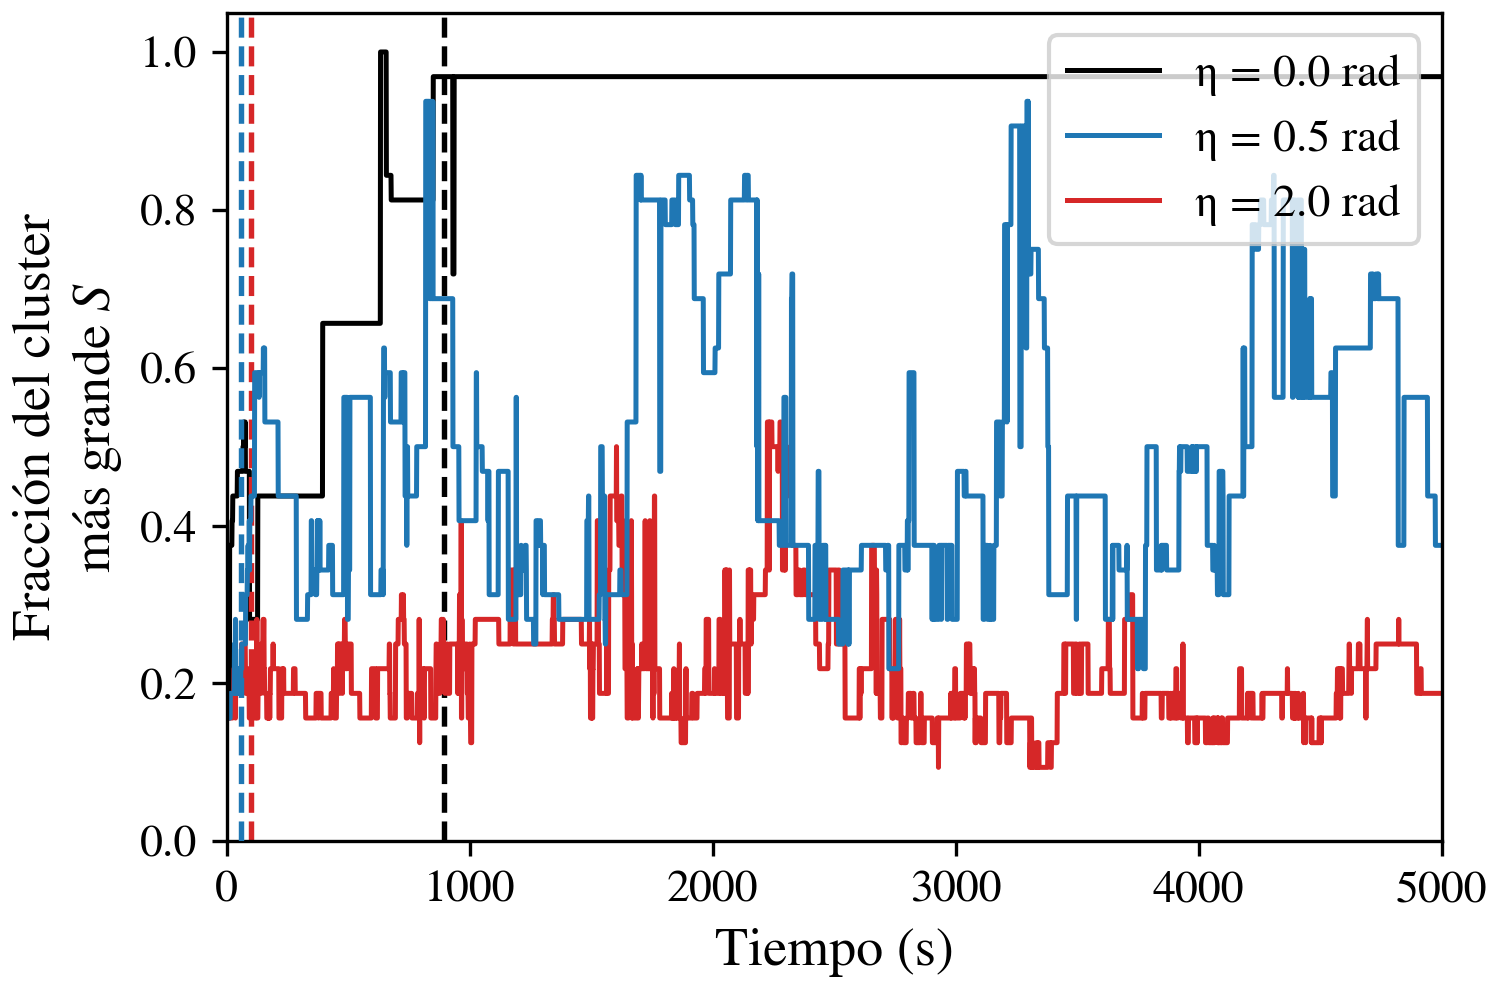
\includegraphics[width=\linewidth]{evolucion_s_voter_rho0.3183.png}\\
        (b) $\rho=1/\pi$.
    \end{minipage}
    \caption{Evolución de la fracción del cluster más grande para el votante.
    Cada panel corresponde a una realización y compara $\eta=0$, $0{,}5$ y
    $2$ rad. Las corridas duran $2000$ s en (a) y $5000$ s en (b), salvo las
    de $\eta=0$, de $10000$ s, de las que se muestra el mismo intervalo.
    Cada línea vertical de trazos marca el comienzo del régimen
    estacionario de la curva de su color; las que empiezan en $t=0$ se
    dibujan levemente corridas para que se distingan. En (a) el eje vertical
    se acotó al intervalo donde varían los datos.}
    \label{fig:evol-s-voter}
\end{figure}

La Fig.~\ref{fig:s-eta-voter} confirma que la densidad domina la conectividad
en los dos modelos. Para $\rho=2$ el mínimo del votante fue
$0{,}98\pm0{,}01$, en $\eta=0{,}5$ rad, y para $\rho=4$ y $8$ superó
$0{,}999$. En las densidades complementarias, $S$ disminuye con el ruido: en
$\rho=1/\pi$ pasó de $0{,}9\pm0{,}2$ en $\eta=0$ a $0{,}16\pm0{,}03$ en
$\eta=6{,}28$ rad, el mismo valor final que en Vicsek.

\begin{figure}[H]
    \centering
    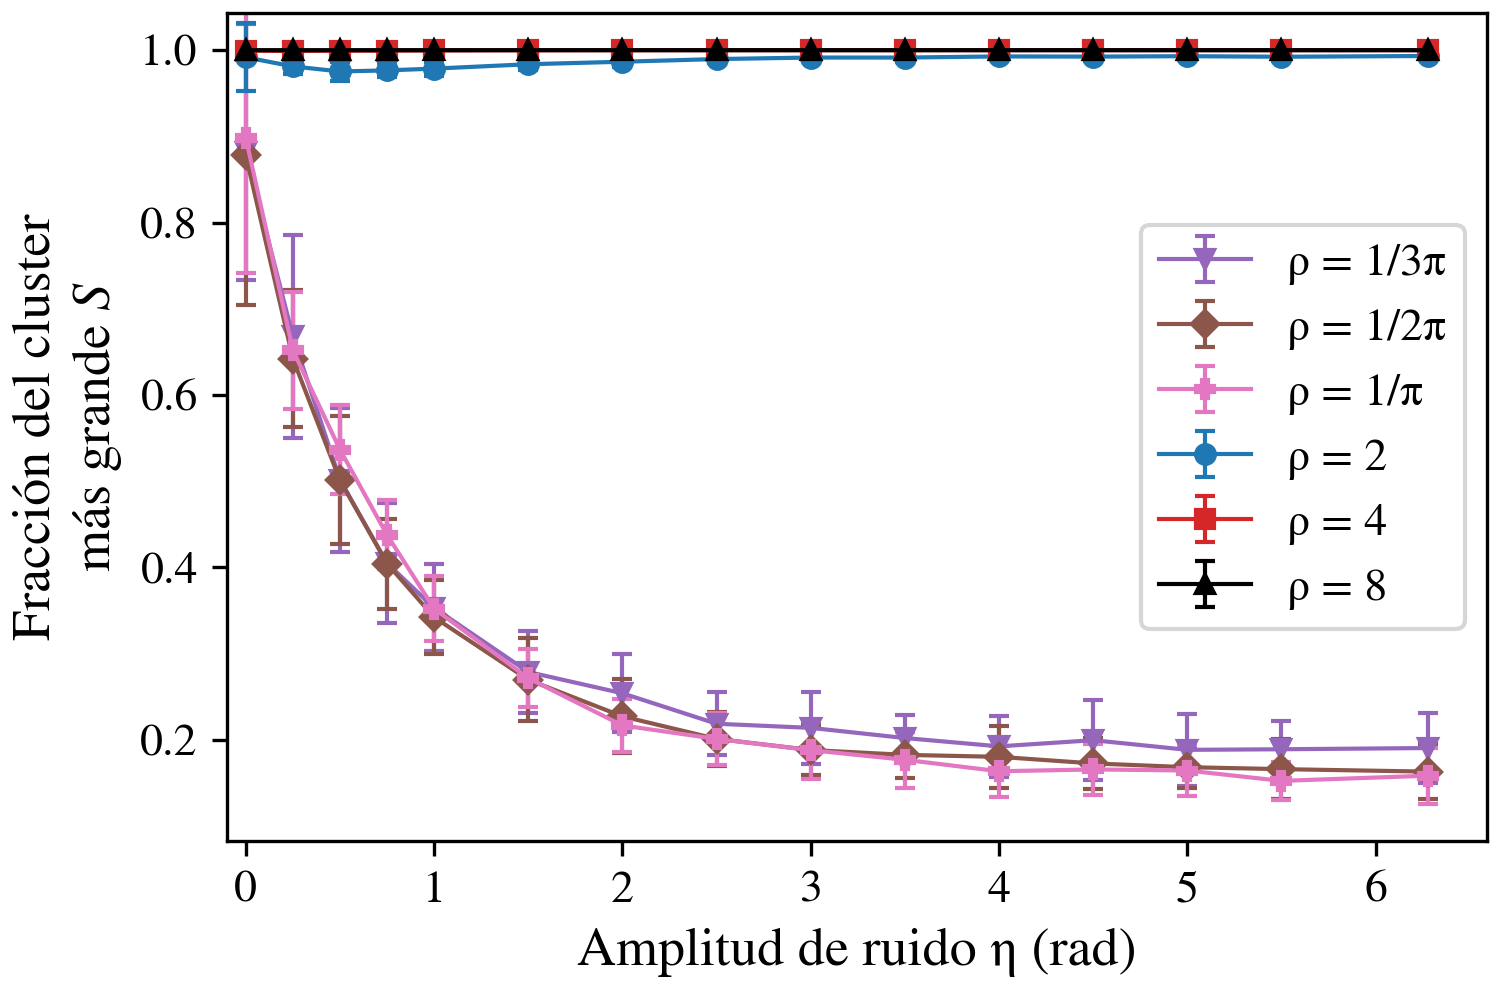
\includegraphics[width=\figw]{voter_s_vs_eta.png}
    \caption{Fracción estacionaria del cluster más grande en función del ruido
    para el modelo de votante.}
    \label{fig:s-eta-voter}
\end{figure}

La Fig.~\ref{fig:comparacion-s-voter} superpone ambos modelos para $\rho=2$,
la densidad principal donde $S$ varía más. Cada modelo tiene un mínimo de $S$
donde cae su polarización: Vicsek baja a $0{,}960\pm0{,}011$ en $\eta=3$ a
$3{,}5$ rad y el votante a $0{,}975\pm0{,}011$ en $\eta=0{,}5$ rad; fuera de
esa zona ambos vuelven a $0{,}99$. La regla de alineación desplaza el mínimo
de $S$ junto con la transición de \va\ (Fig.~\ref{fig:comparacion-va-voter}),
pero la profundidad del mínimo no supera el $4\%$. En $\rho=4$ ocurre lo
mismo con una profundidad de $0{,}2\%$: los mínimos son $0{,}998\pm0{,}001$
en $\eta=3$ rad para Vicsek y $0{,}9990\pm0{,}0006$ en $\eta=0{,}25$ rad para
el votante.

\begin{figure}[H]
    \centering
    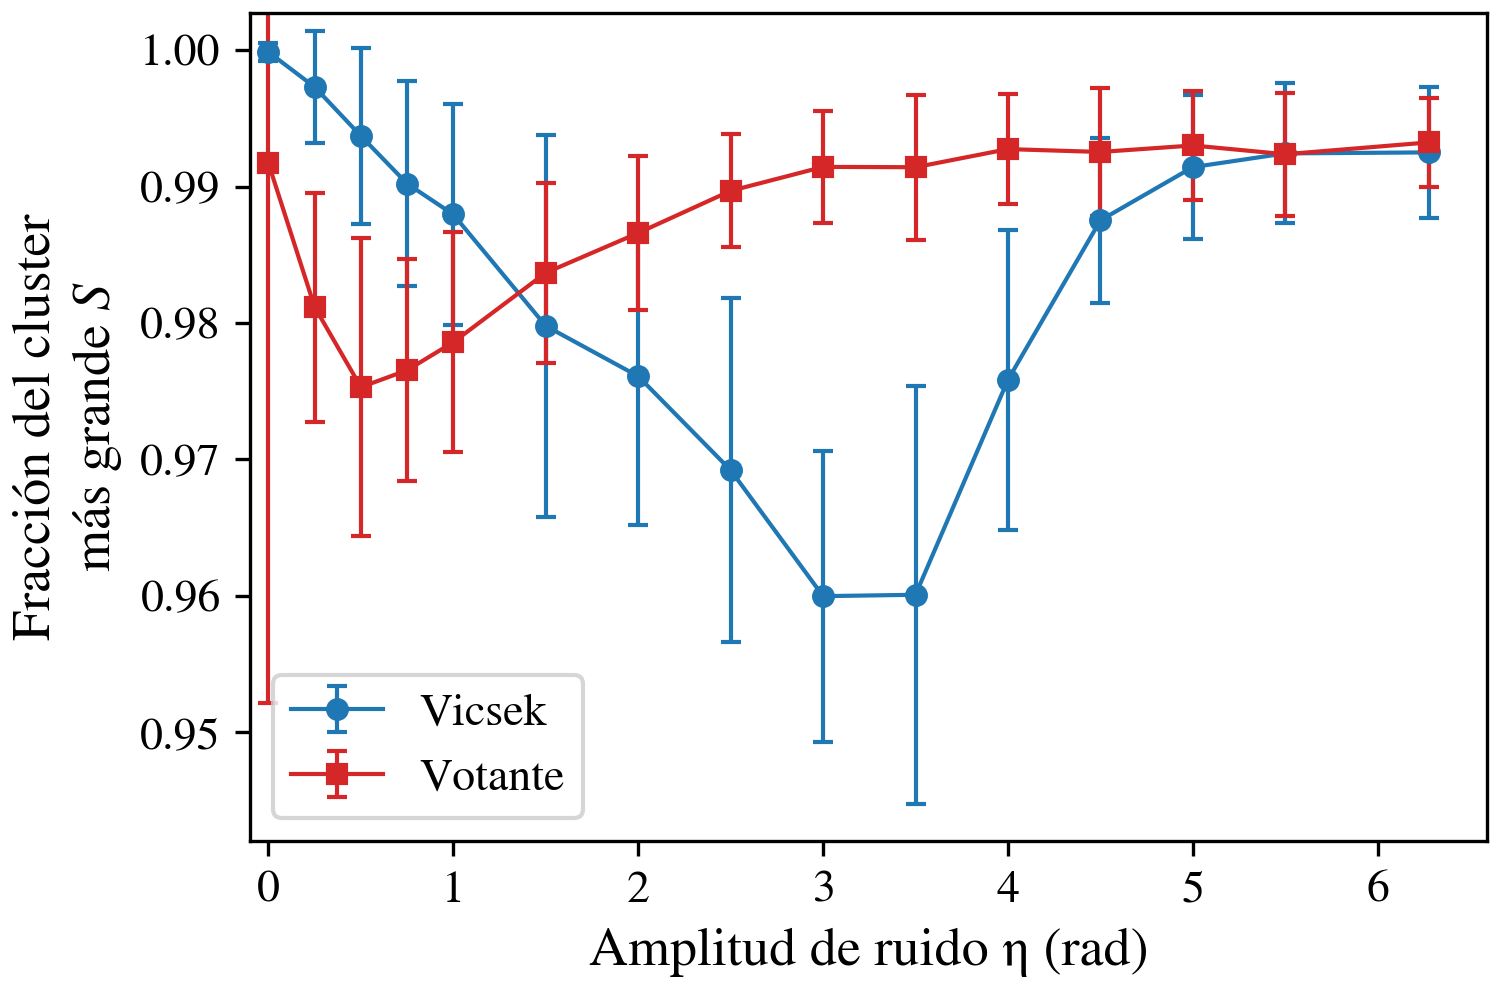
\includegraphics[width=\figw]{comparacion_s_vs_eta_rho2.png}
    \caption{Fracción estacionaria del cluster más grande en función del ruido
    para Vicsek y votante con $\rho=2$. El eje vertical se acotó al intervalo
    donde varían los datos.}
    \label{fig:comparacion-s-voter}
\end{figure}

En la Fig.~\ref{fig:va-s-voter}, las densidades principales vuelven a
concentrarse en $S\simeq1$ para todo el rango de \va, pero con ruidos
intermedios alcanzan polarizaciones menores que en Vicsek. En las densidades
complementarias, \va\ y $S$ presentan una asociación positiva. La comparación
con la Fig.~\ref{fig:va-s-vicsek} muestra que la conectividad espacial es
similar, pero el votante pierde polarización con menor ruido.

\begin{figure}[H]
    \centering
    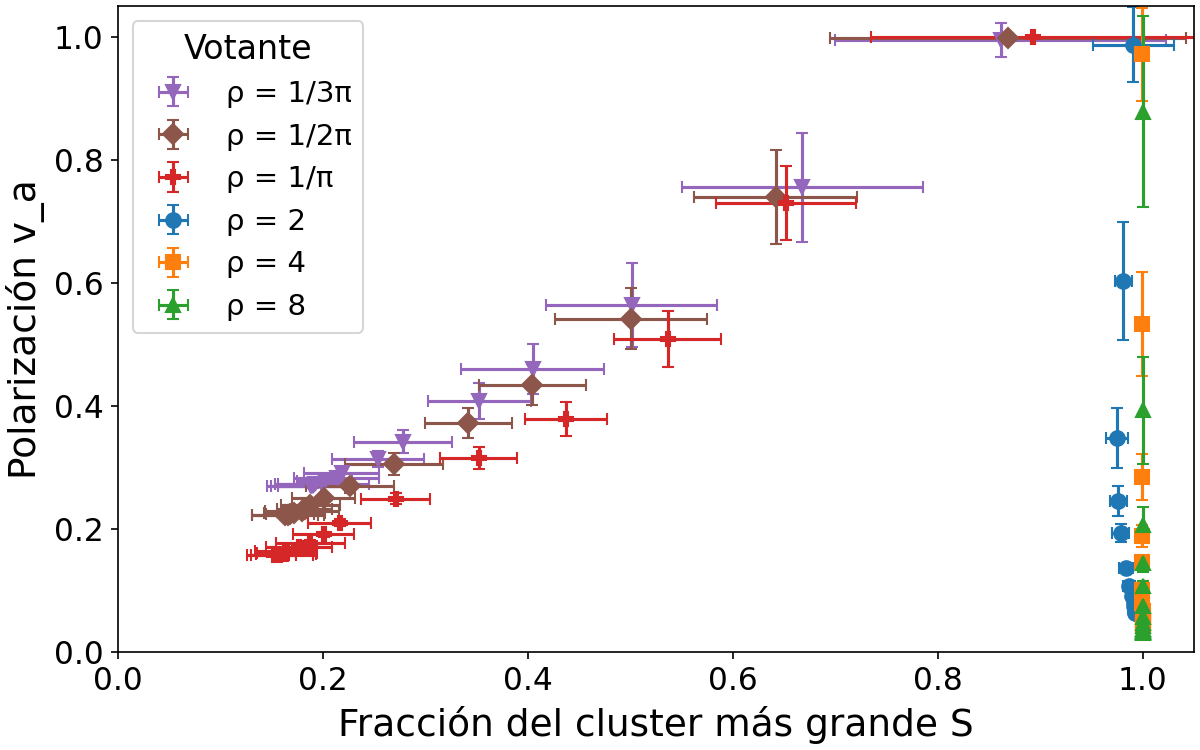
\includegraphics[width=0.88\textwidth]{va_vs_s_voter.png}
    \caption{Polarización en función de la fracción del cluster más grande para
    el votante. La partición en paneles y el significado de las barras son los
    mismos que en la Fig.~\ref{fig:va-s-vicsek}.}
    \label{fig:va-s-voter}
\end{figure}

La Fig.~\ref{fig:comparacion-va-s} cierra la comparación superponiendo ambos
modelos en el plano $\va$--$S$ para una única densidad, $\rho=1/\pi$, la que
recorre el rango más amplio en los dos observables. Las dos curvas se
superponen dentro de sus barras
de error a lo largo de todo el recorrido, desde $(S,\va)\simeq(0{,}16;0{,}16)$
hasta $(0{,}98;1{,}00)$. La regla de alineación no cambia entonces la relación
entre orden y conectividad: los dos modelos recorren el mismo camino y lo único
que cambia es el ruido con el que cada uno llega a cada punto de ese camino,
como muestran las Figs.~\ref{fig:comparacion-va-voter}
y~\ref{fig:comparacion-s-voter}. El detalle por densidad de cada modelo queda
en las Figs.~\ref{fig:va-s-vicsek} y~\ref{fig:va-s-voter}.

\begin{figure}[H]
    \centering
    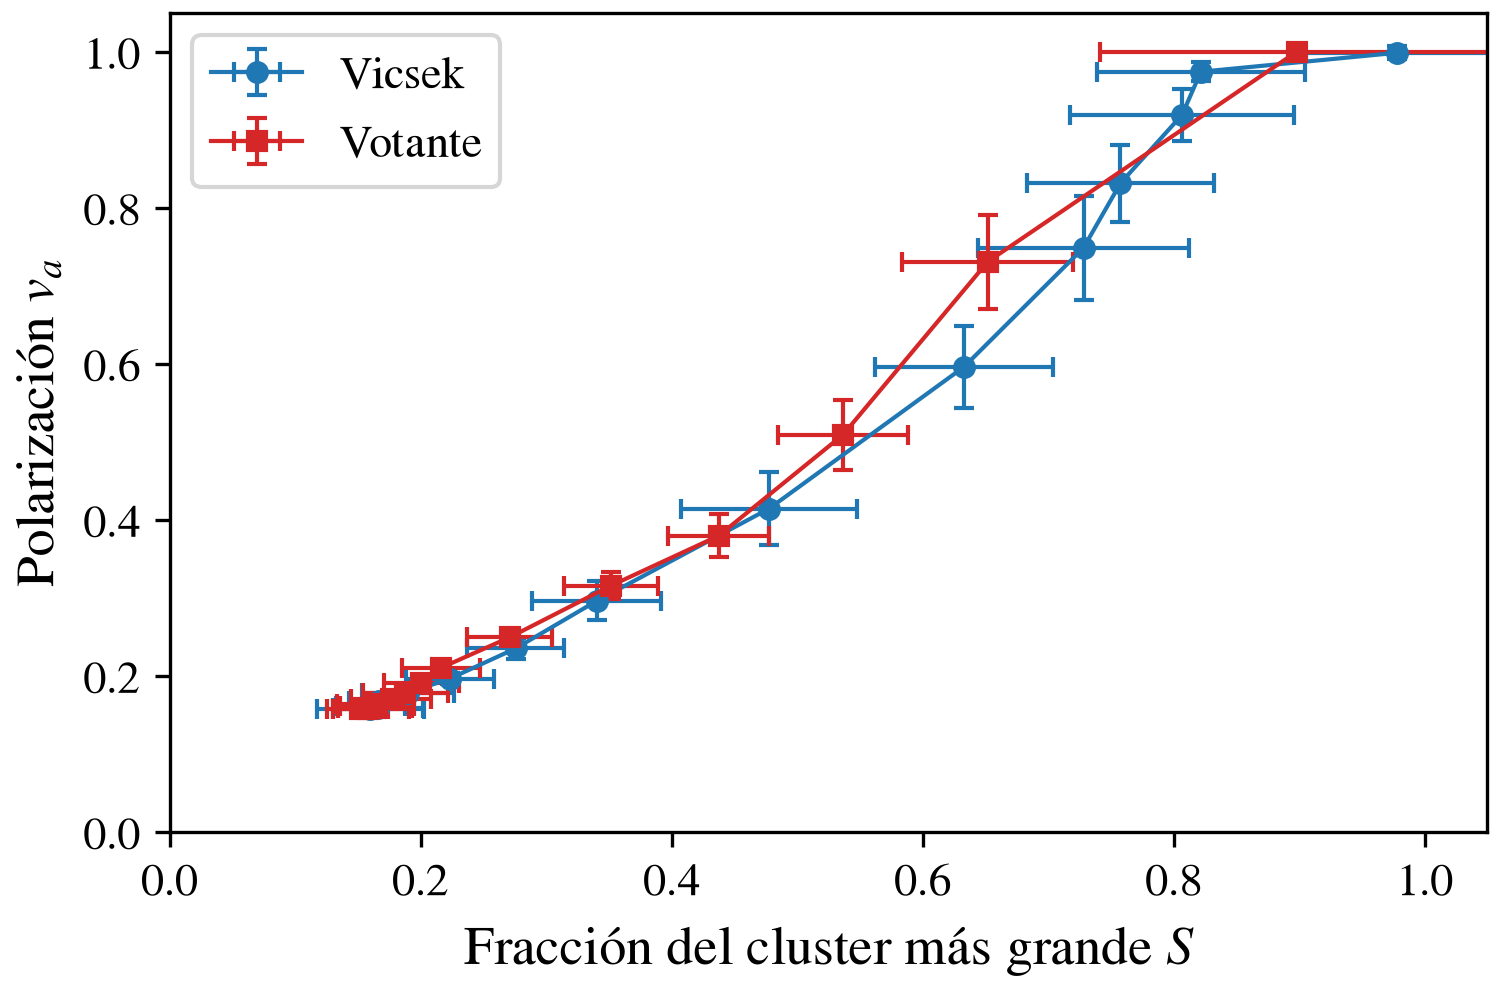
\includegraphics[width=\figw]{comparacion_va_vs_s.png}
    \caption{Polarización en función de la fracción del cluster más grande para
    Vicsek y votante con $\rho=1/\pi$. Cada punto es un valor de ruido y las
    barras son los desvíos estándar de $S$ (horizontales) y \va\
    (verticales).}
    \label{fig:comparacion-va-s}
\end{figure}

\subsection{Tiempos de ejecución del CIM}

Se buscó comprobar si el CIM, aplicado dentro de una simulación real como la
de Vicsek o la del votante, tarda lo mismo por llamada que cuando en el TP1
solo se buscaban vecinos. Las tres series se midieron sobre la misma
geometría ($L=10$ m, $M=10$ celdas por lado, $r_c=1$ m, condiciones
periódicas y partículas puntuales) para $N=200$, $400$ y $800$, es decir
$\rho=2$, $4$ y $8$, con $\eta=0{,}5$ rad en el TP2. La Fig.~\ref{fig:cim}
reúne las tres series.

Los tres casos dan tiempos del mismo orden y con la misma pendiente: en
$N=200$, $0{,}07\pm0{,}01$ ms para Vicsek y $0{,}062\pm0{,}002$ ms para el
votante, contra $0{,}058\pm0{,}009$ ms del TP1. Al multiplicar $N$ por
cuatro, el tiempo por llamada crece un factor entre $10$ y $11$ en los tres.
El crecimiento supera al de $N$ porque $L$ y $M$ se mantienen fijos: al
aumentar $N$ crece la ocupación de cada celda, y con ella la cantidad de
pares que el método revisa por partícula.

El votante coincide con el TP1 dentro de la dispersión en los tres tamaños.
Vicsek queda un $20\%$ por encima en $N=200$ y $400$. La diferencia está en
la configuración sobre la que trabaja el método: con $\eta=0{,}5$ rad Vicsek
forma bandadas, las celdas quedan desbalanceadas y el CIM revisa más pares por
partícula, mientras que a ese ruido el votante casi no se ordena y sus
partículas quedan repartidas de forma uniforme, como en el TP1. Se lo
verificó repitiendo las corridas de Vicsek con $\eta=6{,}28$ rad, donde el
sistema queda desordenado: el tiempo por llamada baja un factor $1{,}4$ en
$N=200$ y $1{,}2$ en $N=800$.

\begin{figure}[H]
    \centering
    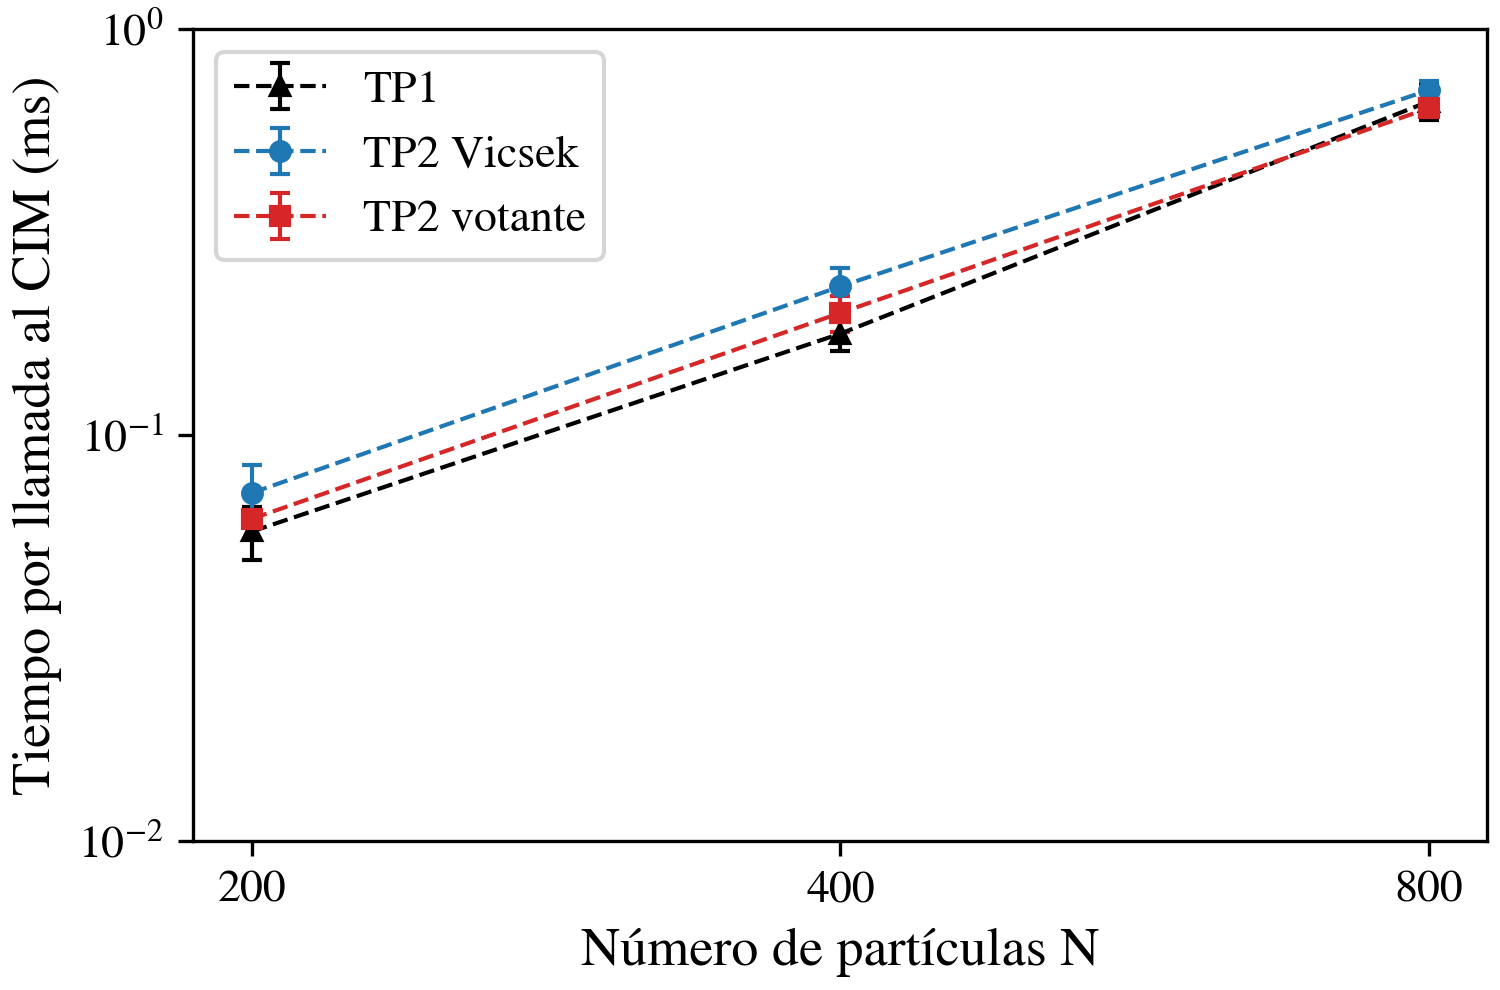
\includegraphics[width=\figw]{cim_tp1_vs_tp2.png}
    \caption{Tiempo por llamada al CIM en función de la cantidad de partículas,
    para la búsqueda de vecinos sola (TP1) y dentro de la simulación de ambos
    modelos (TP2, $\eta=0{,}5$ rad), sobre la geometría común detallada en el
    texto.}
    \label{fig:cim}
\end{figure}

\section{Conclusiones}

El modelo de Vicsek mantuvo valores de polarización cercanos a uno hasta
amplitudes de ruido mayores que el votante, y ese límite se desplazó a ruidos
mayores al aumentar la densidad: en $\eta=3$ rad la polarización fue
$0{,}39\pm0{,}04$; $0{,}54\pm0{,}01$ y $0{,}614\pm0{,}003$ para $\rho=2$,
$4$ y $8$, respectivamente. Para $\rho=4$ pasó de $1{,}000$ sin ruido a
$0{,}783\pm0{,}007$ en $\eta=2$ rad y a $0{,}0443\pm0{,}0008$ en
$\eta=6{,}28$ rad.

El votante fue más sensible al ruido y, a diferencia de Vicsek, aumentar la
densidad hizo caer aún más su polarización. Para $\rho=4$ y $\eta=0{,}25$
rad, su polarización fue $0{,}53\pm0{,}08$, mientras que Vicsek conservó
$0{,}9966\pm0{,}0002$; al pasar de $\rho=2$ a $8$ la polarización del votante
en ese ruido bajó de $0{,}6\pm0{,}1$ a $0{,}39\pm0{,}09$.

La conectividad no siguió la pérdida de orden. Para $\rho=2$, $4$ y $8$, la
fracción del cluster más grande no bajó de $0{,}96$ en ambos modelos, incluso
con el ruido máximo, donde la polarización cayó a $0{,}03$--$0{,}06$. Su
único rasgo es un mínimo en la transición de cada modelo: $0{,}96$ en
$\eta=3$ a $3{,}5$ rad para Vicsek y $0{,}98$ en $\eta=0{,}5$ rad para el
votante, con $\rho=2$. Un único cluster que abarca todo el sistema puede,
por lo tanto, coexistir con movimiento globalmente desordenado.

En las densidades complementarias, $S$ disminuyó con el ruido, de
$0{,}98\pm0{,}08$ a $0{,}16\pm0{,}04$ en $\rho=1/\pi$, y presentó una
asociación positiva con \va. En el plano $\va$--$S$ ambos modelos recorrieron
la misma curva dentro de sus barras de error: la regla de alineación cambia
el ruido al que se llega a cada punto, no la relación entre orden y
conectividad.

El CIM dentro de la simulación tarda lo mismo que en el TP1 para el votante y
un $20\%$ más para Vicsek en $N=200$ y $400$, por el desbalance de celdas que
producen las bandadas.

\phantomsection
\addcontentsline{toc}{section}{Referencias}
\begin{thebibliography}{9}

\bibitem{vicsek1995}
T. Vicsek, A. Czirók, E. Ben-Jacob, I. Cohen y O. Shochet,
``Novel type of phase transition in a system of self-driven particles'',
\textit{Physical Review Letters}, vol. 75, nro. 6, pp. 1226--1229 (1995).

\bibitem{loscar2021}
E. S. Loscar, G. Baglietto y F. Vazquez,
``Noisy multistate voter model for flocking in finite dimensions'',
\textit{Physical Review E}, vol. 104, nro. 3, 034111 (2021).

\end{thebibliography}

\end{document}
